% Created 2025-12-16 Tue 19:31
% Intended LaTeX compiler: pdflatex
\documentclass[11pt]{article}
\usepackage[utf8]{inputenc}
\usepackage{lmodern}
\usepackage[T1]{fontenc}
\usepackage[top=1in, bottom=1.in, left=1in, right=1in]{geometry}
\usepackage{graphicx}
\usepackage{longtable}
\usepackage{float}
\usepackage{wrapfig}
\usepackage{rotating}
\usepackage[normalem]{ulem}
\usepackage{amsmath}
\usepackage{textcomp}
\usepackage{marvosym}
\usepackage{wasysym}
\usepackage{amssymb}
\usepackage{amsmath}
\usepackage[theorems, skins]{tcolorbox}
\usepackage[version=3]{mhchem}
\usepackage[numbers,super,sort&compress]{natbib}
\usepackage{natmove}
\usepackage{url}
\usepackage[cache=false]{minted}
\usepackage[strings]{underscore}
\usepackage[linktocpage,pdfstartview=FitH,colorlinks,
linkcolor=blue,anchorcolor=blue,
citecolor=blue,filecolor=blue,menucolor=blue,urlcolor=blue]{hyperref}
\usepackage{attachfile}
\usepackage{setspace}
\usepackage{tcolorbox}
\usepackage{xcolor} % Needed for defining colors
\definecolor{lightbrown}{RGB}{210,180,140}
\tcbuselibrary{listingsutf8}  % Allows UTF-8 support inside tcolorbox
\tcbset{colback=lightbrown!20, colframe=black, boxrule=0.5pt, arc=3pt, boxsep=5pt}
\definecolor{lightgray}{RGB}{230,230,230}
\tcbset{colframe=black, boxrule=0.5pt, arc=3pt, boxsep=5pt}
\setminted{frame=none}  % Removes horizontal lines
\usepackage[htt]{hyphenat}
\author{Victor Alves and John R. Kitchin}
\date{\today}
\title{Generative machine learning approaches to optimization}
\begin{document}

\maketitle
\tableofcontents

\begin{abstract}
Solving optimization problems, especially for nonlinear and constrained systems, is a challenge. Decades of specialized algorithms have been developed for general and special cases of root finding, minimization (including constraints), for parameter estimation, and mapping connected spaces. These approaches typically require a model, or set of equations, and then analytical, or iterative numerical approaches can be used to find a solution, and in some special cases a globally best solution can be found and proven. In this work we present an alternative approach to solving these problems that is based in generative machine learning models. The idea is these models either estimate a joint probability distribution of input and output variables, or are able to transform a distribution of inputs to a distribution of outputs (or vice versa). Then, by suitable conditioning (specifying desired properties of some variables), the solutions to these problems can be obtained by sampling the distribution, or by transformation of a distribution sample to the solution space. We illustrate the approach with Gaussian mixture models, which approximate the joint probability distribution. We show examples in root finding, unconstrained and constrained optimization, parameter estimation and mapping input and output spaces. This work is intended to be pedagogical to show how a generative model can be used to solve problems in optimization. We discuss some limitations of this approach, but conclude the approach has promise and is different than existing approaches.
\end{abstract}
\section{Introduction}
\label{sec:org1a15650}

The field of optimization is immense, with elegant solutions tailored to specific problem applications, depending on the nature of the objective function and constraints that are to be solved (e.g., linear \emph{vs.} nonlinear, convex \emph{vs.} nonconvex, differentiable \emph{vs.} nondifferentiable), the nature of the variables involved in the optimization problem (discrete, continuous, or both), and lastly, the nature of the solution itself, global \emph{vs.} local optimization. This myriad of problems that arise in many fields of science and engineering gave birth to several solution techniques, ranging from the seminal work of linear programming and the Simplex method by Dantzig \cite{dantzig1990origins}, to the advent of robust nonlinear programming techniques including sequential quadratic programming (SQP) \cite{Han1977,powell_sqp_1978,Wilson1963Simplicial}, and the popularization of interior-point methods \cite{wachter2006implementation}. Additionally, solutions of mixed integer nonlinear programming (MINLP) algorithms \cite{bonami2008} and recent innovations on generalized disjunctive programming (GDP) which embeds logical decisions into mathematical programming formulations \cite{grossmann_gdp}, and global optimization \cite{FLOUDAS20051185,Floudas2009,BOUKOUVALA2016701} are all examples of how rich is the literature on the topic.In Python the \texttt{scipy} library is particularly notable \cite{virtanen-2020-scipy}, but others also exist like \texttt{Pyomo} \cite{bynum-2021-pyomo-optim}, GEKKO \cite{beal-2018-gekko-optim-suite}, Gurobi \cite{gurobi}, Mosek \cite{Andersen2000}, and JuMP \cite{dunning-2017-jump}. These libraries include both algebraic optimization modeling languages as well as commercial and/or open-source optimization solvers. Despite all the work aforementioned, the list is by no means exhaustive, and many other interesting research directions are currently available and being actively developed.

We see a particular interest in algorithmic development of solutions to optimization problems that are specific to the nature of the problem, its variables and local/optimal convergence criteria. However, less attention has been given to the use of emerging and powerful tools such as generative machine learning (genML) in the well-developed area of optimization. It is clear that optimization/mathematical programming is one of the cornerstones of machine learning (independent of the generative nature or lack thereof), but the reverse application, that is, genML as a tool to solve optimization problems, seems to be largely unexplored.

To orient the reader on where a generative-based optimization approach fits in the optimization landscape, we illustrate genML-opt in Figure \ref{fig:opt_flowchart}, based on the classification of optimization problems in Ref. \citenum{biegler2004_retrospective}. We intentionally modified the original flowchart in Refs. \citenum{biegler2004_retrospective,neos_optimization_types}  to show which class of problems we are able to currently employ genML-opt. Although promising, there is still a lot to cover when compared to the current state-of-the-art in optimization.

\begin{figure}[htbp]
\centering
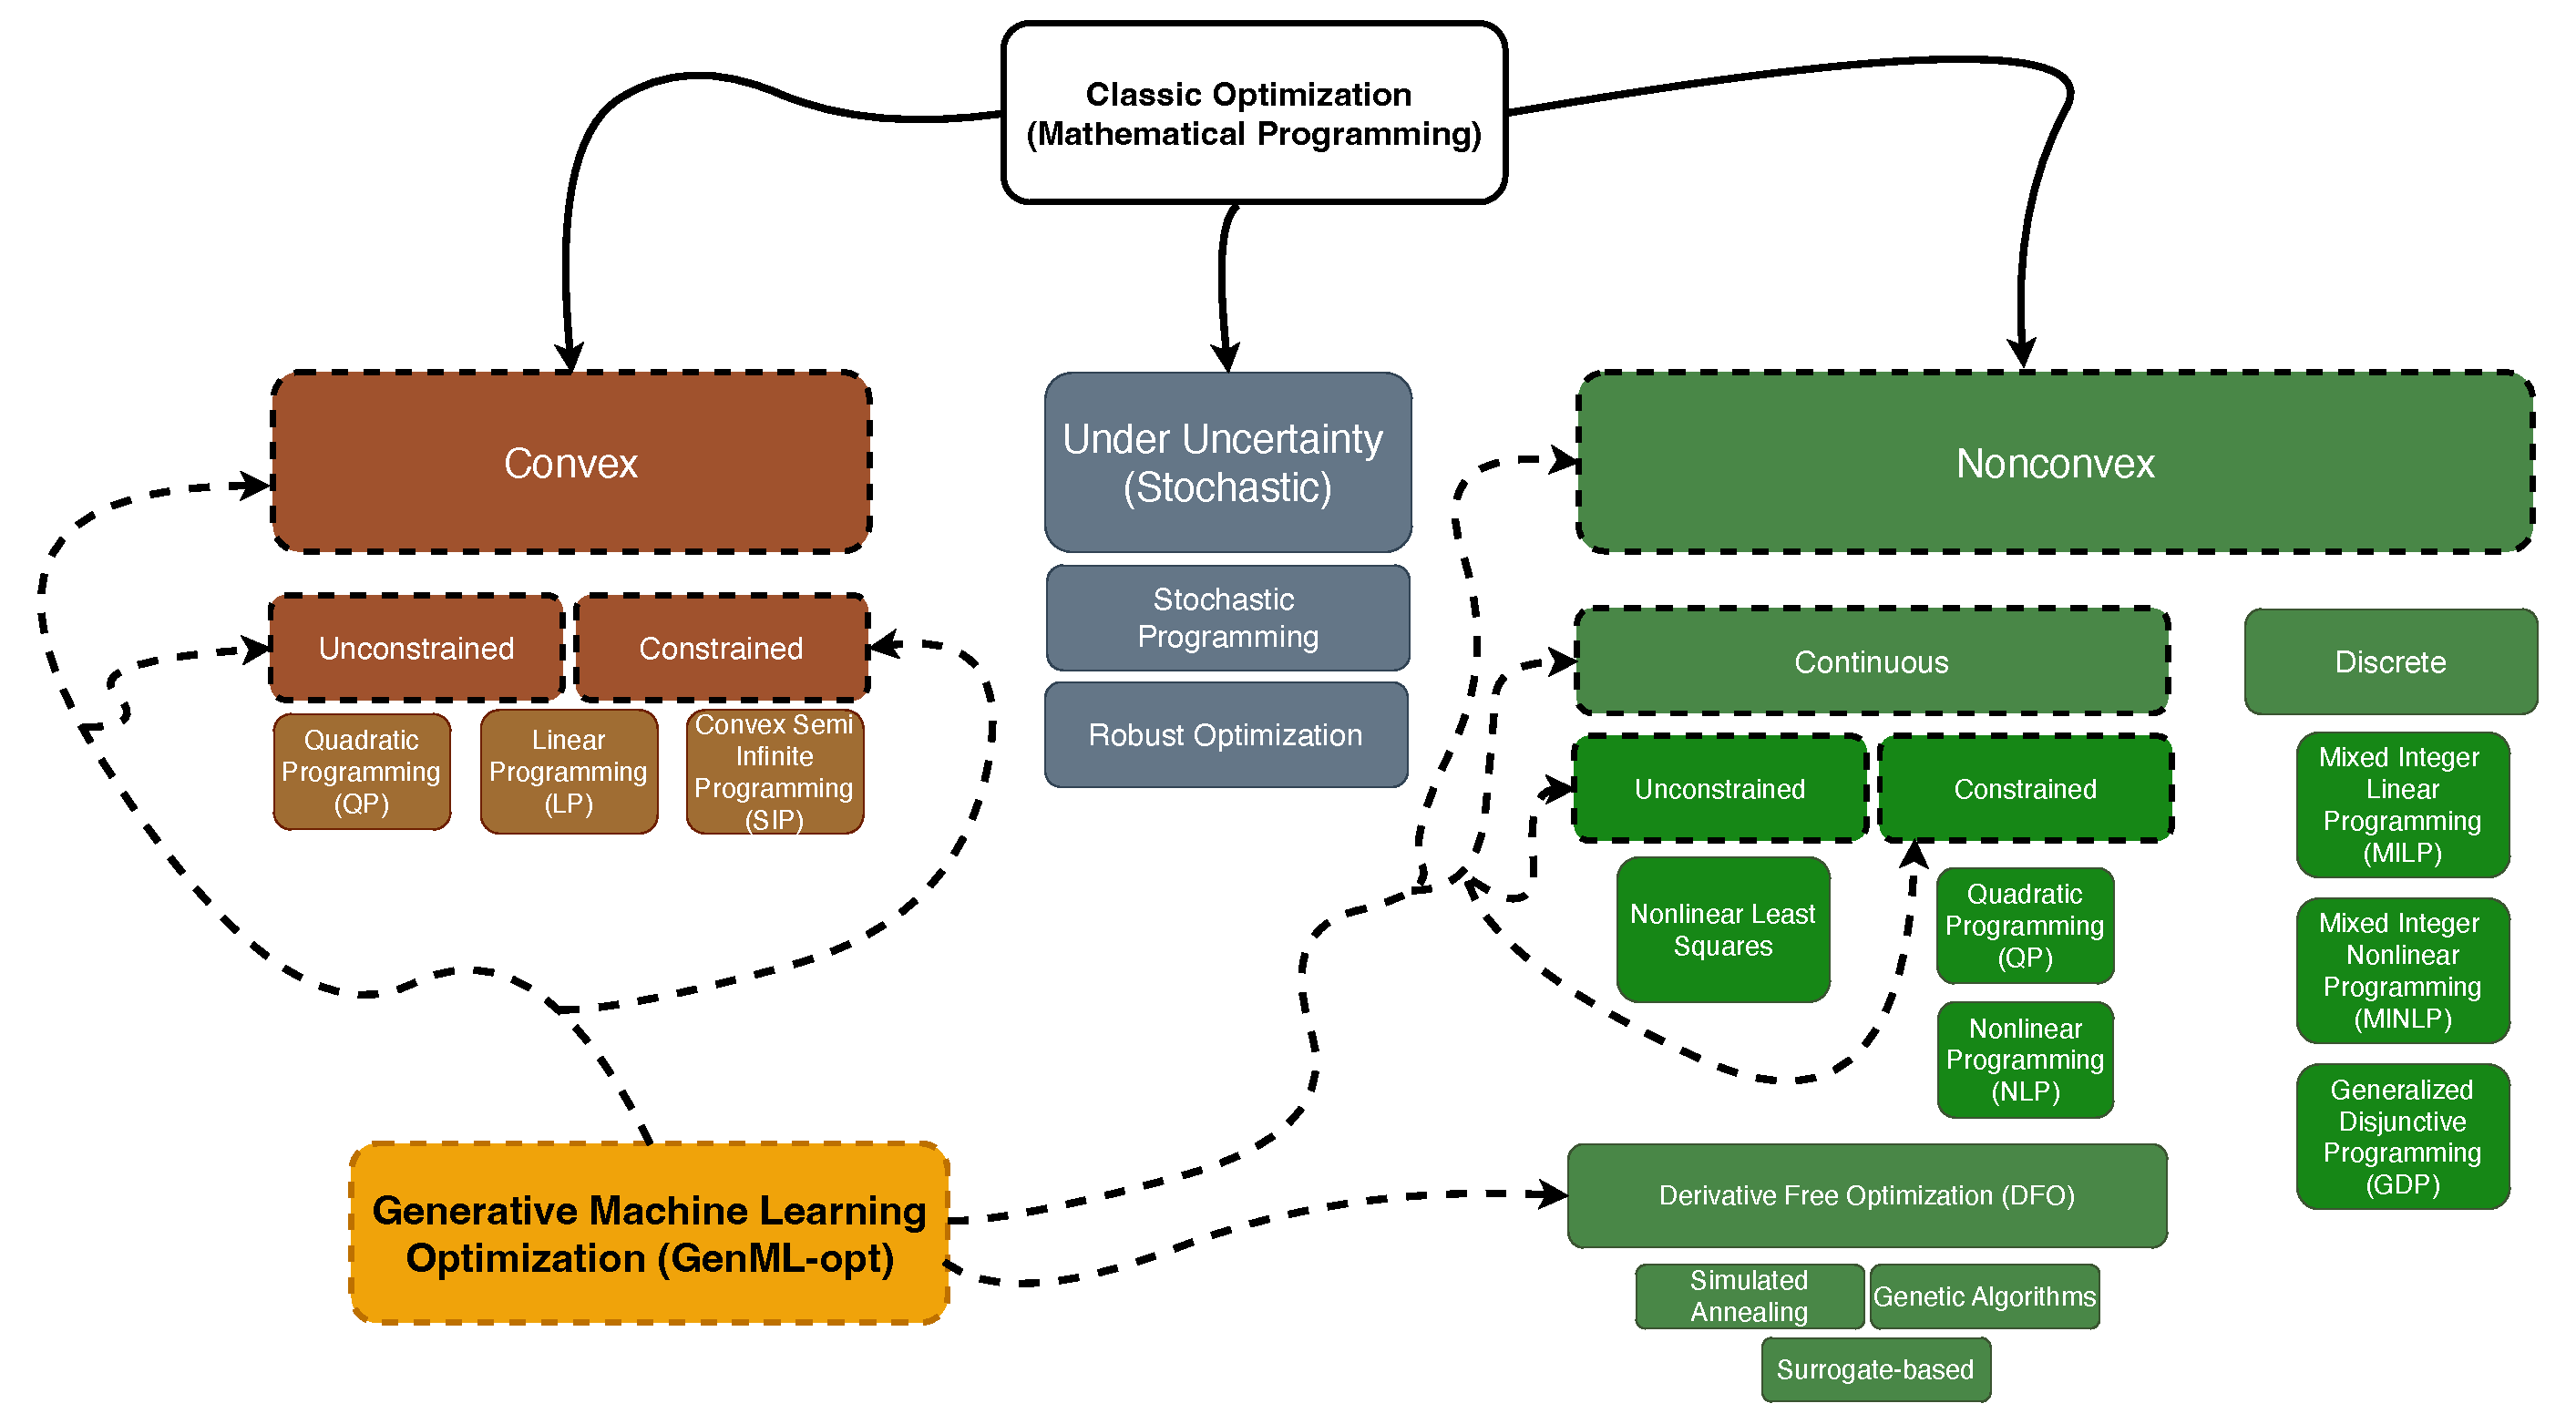
\includegraphics[width=.9\linewidth]{./optimization_flowchart.pdf}
\caption{\label{fig:opt_flowchart}Tree containing classes of optimization problems, based on flowcharts available in the literature \cite{biegler2004_retrospective,neos_optimization_types}. We show with connected dashed lines and also highlighting classes of optimization problems that we were able to currently solve using generative machine learning applied to optimization - GenML-opt.}
\end{figure}

In this manuscript we explore a different way to think about optimization through generative machine learning (genML) \cite{gm-2020-compr-survey}. The basic concept in genML is that if one knows the joint probability distribution of a set of variables, then it is possible to generate samples of that distribution. Alternatively, if one knows how to transform a reference distribution to the joint probability distribution of those variables, then one samples the reference distribution and transforms it to a sample of the desired distribution.

In fact, generative models have been applied to optimization problems before. Invertible neural networks are a special class of models that are used to model the joint distribution of inputs and outputs \cite{ardizzone-2019-analy-inver}. Once they are trained, feasible solutions can be found by sampling them. Diffusion models have been applied to inverse problems in mechanics \cite{dasgupta-2025-condit-score}. We recently applied genML to solve an inverse linear problem \cite{kitchin-2025-solvin}. Generative models can also be used to enhance combinatorial optimization problems \cite{alcazar-2024-enhan-combin} where they can be used to generate near-optimal solutions that are subsequently refined by conventional algorithms. Finally, generative adverserial models have been used in optimization \cite{yao-2024-gener-adver}

Probably the most common genML method used today is in the generation of text \cite{becker-2024-text-gener} and images \cite{elasri-2022-image-gener}. Large language models (LLMs) are a form of genML where the most likely sequence of words to follow a prompt is generated. LLMs are not the focus of this work. In image generation, a genML model is trained on a large set of images to "learn the image distribution", and then images are generated by sampling that distribution. We find it helpful to think of an image first as a matrix of pixel values (e.g. the RGB intensities), and then to think of that matrix as a flattened vector. Then, a large set of images will have a distribution of values in that vector space where there are correlations (covariance) between the elements of the vector that define an image space. Thus, one generates a sample vector, and then reshapes it into a matrix, which can be visualized as an image.  This is the motivation for the present work.

That does not sound immediately helpful in solving optimization problems until we note two things. First, instead of a collection of pixel values, the vector elements  may be inputs and outputs of a model or system, and by concatenating those we obtain a vector analogous to the flattened image vector. The vector elements may even include derivatives of the model, or other easily derived features. If we have a large number of these vectors, then they will form a distribution in that vector space where there are correlations (covariance) between the elements, e.g. the inputs and outputs. Since it is evident generative models can learn that distribution for images, it seems reasonable they could learn this distribution for inputs/outputs, which we demonstrate in this work.

Thus, if we can learn or estimate the joint probability distribution, we can generate samples of inputs and outputs from it. Second, we must introduce the idea of conditional generation, that is, we can specify some values of the variables, update the joint probability distribution of the remaining variables, and then generate those variables consistent with our condition. Thus, if we condition on inputs, we can then generate samples of the output, and vice versa. This is directly related to root finding; we might condition on the output being zero, and generate the inputs that lead to that result.

To connect this idea to finding minima/maxima we simply need to see the connection between inputs of a model and its derivatives. If we know that joint probability distribution, then we generate samples conditioned on the derivatives being equal to zero. We can include constraints by leveraging a Lagrangian function, or another augmented function and condition the derivatives of that to be zero. Finally, in parameter estimation, we need the joint probability distribution between the parameters and an observed output(s). Then to estimate parameters from an observation, we simply condition on the observation to find the parameters. These are all related to solving inverse problems in optimization.

We think this approach is fundamentally different than a conventional view point. There may be a model involved, but it is not necessary; the approach can be completely data-driven in some cases. We do not need to think about a forward or inverse model. The joint probability distribution (or the transformation function) is simultaneously both of these; conditioning determines what direction if any one thinks in (for example, it is possible to condition on some inputs and outputs). That means we get solutions to optimization problems without using conventional approaches like Newton-Raphson iterative methods, or other specialized algorithms like simplex methods to solve nonlinear programs. We make no claims of superiority of generative methods over the well-established methods; indeed, conventional algorithms offer many advantages to the ideas presented here. Instead, we focus on developing a proof of concept for a new way to think about solving these problems. We do this through a series of examples that span root finding, minimization including constraints, parameter estimation, and state mapping.

GenML has the potential to serve as an alternative optimization solution approach to several classes of problems listed above, including linear and nonlinear programming (both constrained and unconstrained), parameter estimation problems, inverse mapping, and root finding, to name a few. Intriguingly, we have observed that the solution approach to these types of problems is remarkably consistent, as opposed to highly-tailored and specific algorithms (the current \emph{status quo}) as long as data is available. We do not anticipate that generative machine learning formulations will replace classic mathematical programming development. Instead, we believe that a branch of optimization problems that can be solved by using GenML will employ even more sophisticated optimization algorithms at the training and inference of generative models. In short, the optimization layer will always be present, and its interaction with the researcher/practitioner will be what might change within the next years.
\section{Methods}
\label{sec:orgb943650}

We will focus on Gaussian Mixture Models (GMM) in this work, particularly an implementation in \texttt{gmr} \cite{fabisch-2021-gmr}. There are other generative models based on diffusion and continuous flow matching \cite{jolicoeur-martineau-2023-gener-imput} that also work, but for the purpose of this paper, they function practically the same. Analogous to the "no free lunch" theorem, there is no one-size-fits all generative model; but, with enough data and training, they all perform the same on average \cite{wolpert-1997-no-free}. This is analogous to it not mattering whether one chooses a neural network or Gaussian process model; with enough data they are are both useful, and the choice is often made out of convenience or preference.
\subsection{Gaussian mixture models}
\label{sec:org0e2d953}

Gaussian Mixture Models (GMMs) are a powerful and versatile mathematical tool that is able to characterize complex and multimodal distributions by combining multiple individual Gaussians. They are used in machine learning applications related but not limited to data clustering \cite{Yang_2019_ICCV,viroli_deep_2019}. They are also recognized in the literature related to pattern recognition in machine learning \cite{bishop2006pattern}. Furthermore, in the field of robotics, Gaussian Mixture Regression (GMR) has been used as a generative modeling framework  \cite{Fabisch2021},  and it is considered a generative model \cite{deisenroth2020mathematicsML}. We follow the notation from Ref \citenum{Fabisch2021} for the mathematical definition of GMMs. However, the reader should note that equally valid formulations are present in the literature \cite{deisenroth2020mathematicsML,bishop2006pattern}.

From a machine learning perspective, the main task is, given a pair of vectors \(x\) and \(y\), to learn a probability distribution as defined as in Eq. \ref{eq:GMM_01}, which is the definition of a Gaussian mixture model.


\begin{equation} \label{eq:GMM_01}
p(\boldsymbol{x}, \boldsymbol{y})=\sum_{k=1}^K \pi_k \mathcal{N}_k\left(\boldsymbol{x}, \boldsymbol{y} \mid \boldsymbol{\mu}_{\boldsymbol{x} \boldsymbol{y}_k}, \boldsymbol{\Sigma}_{\boldsymbol{x} \boldsymbol{y}_k}\right)
\end{equation}

\noindent In which \(\mathcal{N}_k\left(\boldsymbol{x}, \boldsymbol{y} \mid \boldsymbol{\mu}_{\boldsymbol{x} \boldsymbol{y}_k}, \boldsymbol{\Sigma}_{\boldsymbol{x} \boldsymbol{y}_k}\right)\) are the \(k^{th}\) Gaussian distributions in a mixture, which are defined by their respective means \(\boldsymbol{\mu}_{\boldsymbol{x} \boldsymbol{y}_k}\) and covariances \(\boldsymbol{\Sigma}_{\boldsymbol{x} \boldsymbol{y}_k}\). \(\pi_k \in [0,1]\) are defined as \textit{weights} or \textit{priors}, which quantify the contribution of each Gaussian to the mixture model.
\subsubsection{Training}
\label{sec:org8d8d17d}

The training step corresponds to obtaining an accurate prediction of this unknown, probably multimodal and multivariable probability distribution, given a dataset defined by the pair of vectors \(x,y\). For simplicity, we can lump the parameters related to the formulation of Eq. \ref{eq:GMM_01} which includes the means, covariances and mixture weights as \(\theta := \left\{\pi_k, \boldsymbol{\mu}_{\boldsymbol{x} \boldsymbol{y}_k}, \boldsymbol{\Sigma}_{\boldsymbol{x} \boldsymbol{y}_k}: k=1, \ldots, K\right\}\)

As a figure of merit is needed to fit this generative machine learning model, we resort to a likelihood formulation, defined as in Eq.\ref{eq:logLL}

\begin{equation} \label{eq:logLL}
p(x,y \mid \boldsymbol{\theta})=\prod_{n=1}^N p\left(x_n,y_n \mid \boldsymbol{\theta}\right), \quad p\left(x_n,y_n \mid \boldsymbol{\theta}\right)=\sum_{k=1}^K \pi_k \mathcal{N}\left(x,y \mid \boldsymbol{\mu}_k, \boldsymbol{\Sigma}_k\right)
\end{equation}

The log-likelihood \cite{deisenroth2020mathematicsML} is formulated in Eq.\ref{eq:logLL_2}. Ideally, one could solve for \(\mathrm{d} \mathcal{L} / \mathrm{d} \boldsymbol{\theta} = 0\) and the optimal parameters \(\theta^*\) that maximizes the likelihood would be obtained analytically. However, since Eq. \ref{eq:logLL_2} is not a closed-form expression/solution \cite{deisenroth2020mathematicsML}, an iterative method is used. Expectation Maximization (EM) is applied in GMMs sucessfully and this is what packages such as \texttt{gmr} \cite{Fabisch2021} and the scikit-learn \cite{scikit-learn} implementation of GMM does.

\begin{equation} \label{eq:logLL_2}
\log p(\boldsymbol{x,y} \mid \boldsymbol{\theta})=\sum_{n=1}^N \log p\left(\boldsymbol{x}_n \mid \boldsymbol{\theta}\right)=\underbrace{\sum_{n=1}^N \log \sum_{k=1}^K \pi_k \mathcal{N}\left(\boldsymbol{x}_n \mid \boldsymbol{\mu}_k, \boldsymbol{\Sigma}_k\right)}_{=: \mathcal{L}}
\end{equation}
\subsubsection{Prediction}
\label{sec:orgfc000df}

Following the conditional distribution property of each individual Gaussian, one is able to compute the conditional distribution \(p(y \mid x,\theta)\) by first writing down the conditional distribution for a given \(k^{th}\) element \cite{Fabisch2021}.

\begin{equation}
\boldsymbol{\mu}_{\boldsymbol{xy}_k} =
\begin{bmatrix}
\boldsymbol{\mu}_{\boldsymbol{x}k} \\
\boldsymbol{\mu}_{\boldsymbol{y}k}
\end{bmatrix},
\quad
\boldsymbol{\Sigma}_{\boldsymbol{xy}_k} =
\begin{bmatrix}
\boldsymbol{\Sigma}_{\boldsymbol{xx}_k} & \boldsymbol{\Sigma}_{\boldsymbol{xy}_k} \\
\boldsymbol{\Sigma}_{\boldsymbol{yx}_k} & \boldsymbol{\Sigma}_{\boldsymbol{yy}_k}
\end{bmatrix}
\end{equation}

\noindent The conditional distribution of \(\boldsymbol{y}\) given \(\boldsymbol{x}\) for the \(k^{th}\) Gaussian component is defined as in Eq.\ref{eq:GMM_cond_01}:

\begin{equation} \label{eq:GMM_cond_01}
\begin{aligned}
\boldsymbol{\mu}_{\boldsymbol{y} \mid \boldsymbol{x}}^{(k)} &= \boldsymbol{\mu}_{\boldsymbol{y}k} + \boldsymbol{\Sigma}_{\boldsymbol{yx}_k} \boldsymbol{\Sigma}_{\boldsymbol{xx}_k}^{-1}(\boldsymbol{x} - \boldsymbol{\mu}_{\boldsymbol{x}k}) \\
\boldsymbol{\Sigma}_{\boldsymbol{y} \mid \boldsymbol{x}}^{(k)} &= \boldsymbol{\Sigma}_{\boldsymbol{yy}_k} - \boldsymbol{\Sigma}_{\boldsymbol{yx}_k} \boldsymbol{\Sigma}_{\boldsymbol{xx}_k}^{-1} \boldsymbol{\Sigma}_{\boldsymbol{xy}_k}
\end{aligned}
\end{equation}

To obtain the full conditional distribution \(p(\boldsymbol{y} \mid \boldsymbol{x})\), we combine the component-wise conditional Gaussians using the posterior weights \(\pi_{k \mid \boldsymbol{x}}\), which represent the probability of component \(k\) given the observed \(\boldsymbol{x}\):

\begin{equation}
\pi_{k \mid \boldsymbol{x}} = \frac{\pi_k \, \mathcal{N}(\boldsymbol{x} \mid \boldsymbol{\mu}_{\boldsymbol{x}k}, \boldsymbol{\Sigma}_{\boldsymbol{xx}_k})}{\sum_{l=1}^K \pi_l \, \mathcal{N}(\boldsymbol{x} \mid \boldsymbol{\mu}_{\boldsymbol{x}l}, \boldsymbol{\Sigma}_{\boldsymbol{xx}_l})}
\end{equation}

Finally, the final predicted distribution corresponds to a mixture of conditional Gaussians:

\begin{equation}
p(\boldsymbol{y} \mid \boldsymbol{x}) = \sum_{k=1}^K \pi_{k \mid \boldsymbol{x}} \, \mathcal{N}(\boldsymbol{y} \mid \boldsymbol{\mu}_{\boldsymbol{y} \mid \boldsymbol{x}}^{(k)}, \boldsymbol{\Sigma}_{\boldsymbol{y} \mid \boldsymbol{x}}^{(k)})
\end{equation}

If one desires to have them in a more compact form, we refer to our previous definition of the lumped hyperparameters as \(\theta\) as

\begin{equation}
    \theta =: \left\{ \pi_k, \boldsymbol{\mu}_{\boldsymbol{x} \boldsymbol{y}_k}, \boldsymbol{\Sigma}_{\boldsymbol{x} \boldsymbol{y}_k} \right\}_{k=1}^K
\end{equation}


\noindent which yields a predictive distribution form as in Eq. \ref{eq:GMM_predict_compact}.

\begin{equation} \label{eq:GMM_predict_compact}
p(\boldsymbol{y} \mid \boldsymbol{x}; \theta) = \sum_{k=1}^K \pi_{k \mid \boldsymbol{x}}(\theta) \, \mathcal{N}(\boldsymbol{y} \mid \boldsymbol{\mu}_{\boldsymbol{y} \mid \boldsymbol{x}}^{(k)}, \boldsymbol{\Sigma}_{\boldsymbol{y} \mid \boldsymbol{x}}^{(k)})
\end{equation}


Eq. \ref{eq:GMM_predict_compact} plays a major role in our work. As we draw samples based on conditioning, we can simultaneously infer in variables that belong to both the \(x\) or \(y\) spaces. We show this in several applications related to optimization.

Lastly, we note that typical optimization techniques are used, more specifically during the training step of the generative approach, namely the EM algorithm \cite{nips1993_EM}. However, this optimization step that requires \(\mathcal{O}(\mathcal{D}^3)\) for a dataset of dimensionality \(\mathcal{D}\), is performed offline and separately from the applications in which the GM model is employed.
\subsection{Utility functions}
\label{sec:org7e62e6a}

We do have to do some hyperparameter tuning with a GMM, most notably choosing the number of components in the model. To avoid a lot of duplicated code in this work, we develop this function to automate that choice for us based on an information criteria. This function uses Bayesian Information Criteria (BIC) to pick the best GMM for a given data set.

\begin{minted}[frame=lines,fontsize=\scriptsize,linenos=]{python}
from sklearn.mixture import GaussianMixture
import numpy as np
from gmr import GMM

def best_gmm_bic(X, maxN=None):
    """
    Find the best Gaussian Mixture Model (GMM) for the given data.

    This function uses the Bayesian Information Criterion (BIC) to evaluate
    the fit of Gaussian Mixture Models with varying number of components, and
    returns the model with the lowest BIC value.

    Parameters
    ----------
    X : array-like, shape (n_samples, n_features)
        The input data to be modeled by the GMM.

    maxN : int, optional
        The maximum number of components to consider for the GMM.
        If None, a default value will be used.

    Returns
    -------
    best_gmm : GaussianMixture
        The Gaussian Mixture Model with the lowest BIC for the given data.

    """

    bics = []
    models = []

    for k in range(1, min(100, maxN or(len(X)))):
        model = GaussianMixture(n_components=k,
                                covariance_type='full',
                                random_state=0).fit(X)

        gmm = GMM(n_components=model.n_components,
                  priors=model.weights_,
                  means=model.means_,
                  covariances=model.covariances_)

        bics.append(model.bic(X))
        models.append(gmm)

    best_k = np.argmin(bics)
    model = models[best_k]

    model.models = models
    model.bics = bics

    return model
\end{minted}

We will also need a convenient way to analyze clusters of samples. We use a density-based clustering algorithm to identify the clusters, and then do statistical analysis on those clusters.

\begin{minted}[frame=lines,fontsize=\scriptsize,linenos=]{python}
from sklearn.cluster import DBSCAN

def cluster_stats(X):
    """Compute mean and stdev for clusters in an array.

    This function is used for the side-effect of printing those results.

    Parameters
    ----------
    X : array-like

    Returns
    -------
    None

    """
    X = np.atleast_2d(X)
    clustering = DBSCAN().fit(X)
    labels = clustering.labels_

    for L in set(labels):
        mean = np.mean(X[labels == L])
        std = np.std(X[labels == L])
        n = len(X[labels == L])
        print(f'{L:3d}: {mean: 5.3f} +\\- {std:1.4f} (n={n})')
\end{minted}

It is convenient to set some default parameters for figures here. These settings make the figures transparent and higher resolution.

\begin{minted}[frame=lines,fontsize=\scriptsize,linenos=]{python}
import matplotlib as mpl

mpl.rcParams['figure.facecolor'] = 'none'
mpl.rcParams['axes.facecolor'] = 'none'
mpl.rcParams['figure.dpi'] = 300  # Set DPI to 300
\end{minted}
\section{Results and discussion}
\label{sec:org907e99c}
\subsection{Root finding  \label{sec-root-finding}}
\label{sec:org5e7d0a2}

In root finding we seek to find the values of \(x\) where \(f(x)=0\). We demonstrate this first on a polynomial where there are two real and two imaginary roots. We start by creating data that represent samples of \(x\) and the corresponding values of \(y\). This data is sampled from a function, but it could also be observation data from an instrument, for example. Here we consider a polynomial \(y = x^4 - 4x^2 + x + 3\). This function has easily computable roots for comparison with the roots we subsequently obtain by a generative model. We find those roots next with a conventional function \texttt{numpy.roots}.

\begin{minted}[frame=lines,fontsize=\scriptsize,linenos=]{python}
import numpy as np
import matplotlib.pyplot as plt

x = np.linspace(-2.25, 2, 200)
y = x**4 - 4*x**2 + x + 3
np.roots([1, 0, -4, 1, 3])
\end{minted}

\phantomsection
\label{}
\begin{verbatim}
array([ 1.36778435+0.23154129j,  1.36778435-0.23154129j,
       -1.92630322+0.j        , -0.80926547+0.j        ])
\end{verbatim}


There are two real roots to this equation at \(x\approx-1.93, -0.81\). We can see these roots here:

\begin{minted}[frame=lines,fontsize=\scriptsize,linenos=]{python}
plt.plot(x, y, label='f(x)')
plt.plot([-1.92630322, -0.80926547], [0, 0], 'ro', label='real roots')
plt.axhline(0, color='k', ls='--')
plt.xlabel('x')
plt.legend()
plt.ylabel('y');
\end{minted}

\begin{center}
\includegraphics[width=.9\linewidth]{./.ob-jupyter/a1e6c4878ad1f10a91ee8369cbd19698cb8af456.png}
\label{}
\end{center}


To solve this with a generative approach, we first build a generative model.  It is tricky to evaluate the goodness of fit in a GMM model. Here we plot predictions with the data for a visual comparison. One can use parity plots, R\textsuperscript{2}, MAE, RMSE, and others. We show some of these here. Close inspection of the red predicted line shows some fitting artifacts in the minima and maxima. These do not impact the current problem as they are not near the roots we seek. One could even eliminate that data points where \(y\) is not close to zero here.

\begin{minted}[frame=lines,fontsize=\scriptsize,linenos=]{python}
data = np.array([x, y]).T

gmm = best_gmm_bic(data)
pred = gmm.predict([0], data[:, 0:1])

known_y = data[:, 1]
pred_y = pred[:, 0]

R2 = 1 - np.sum((known_y - pred_y)**2) / np.sum((known_y - np.mean(known_y))**2)

print(f'R2 = {R2:1.3f}')
print(f'MAE = {np.mean(np.abs(known_y - pred_y)):1.2f}')

plt.plot(data[:, 0], data[:, 1], 'b.', label='true')
plt.plot(data[:, 0], pred[:, 0], 'r-', label='predicted')
plt.xlabel('x')
plt.ylabel('y')
plt.axhline(0, c='k', ls='--')
plt.legend();
\end{minted}

\phantomsection
\label{}
\begin{verbatim}
R2 = 1.000
MAE = 0.02
\end{verbatim}

\begin{center}
\includegraphics[width=.9\linewidth]{./.ob-jupyter/1cde2744d7c3481b05b60eb4b69d116d398d0618.png}
\end{center}

That model fit seems reasonable. Now, we just generate conditional samples for \(y=0\). We can compute the conditional probability density for that condition. Here we can see the probability density is basically zero except for two places that are near the two real roots.

\begin{minted}[frame=lines,fontsize=\scriptsize,linenos=]{python}
# the first argument is the indices to condition on
# the second argument is the value to condition those variables.
# Here x is in index 0, and y is in index 1; [x, y]
c = gmm.condition([1], [[0.0]])
# compute conditional probability that each x corresponds to a value of y=0.0
_x = np.linspace(-2, 2, 1000)[:, None]

plt.plot(_x, c.to_probability_density(_x))
plt.xlabel('x')
plt.ylabel('Conditional probability density');
\end{minted}

\begin{center}
\includegraphics[width=.9\linewidth]{./.ob-jupyter/1de421721615e80b6be85d4ea150a1dcbae7b63f.png}
\label{}
\end{center}


To see a more quantitative result, we have to sample the model many times, and evaluate statistics. Note that this model ends up producing two primary values that correspond to the roots. There is some uncertainty in these values because the model does not fit the data perfectly. That is a limitation of the GMM; there is no noise in our function evaluations.

\begin{minted}[frame=lines,fontsize=\scriptsize,linenos=]{python}
cluster_stats(c.sample(1000))
\end{minted}

\phantomsection
\label{}
\begin{verbatim}
 0: -1.926 +\- 0.0018 (n=310)
 1: -0.809 +\- 0.0012 (n=689)
-1:  1.377 +\- 0.0000 (n=1)
\end{verbatim}


Similar to using \texttt{scipy.optimize.root}, we cannot find the imaginary roots by sampling real values, and we show how to resolve this in the next section. We note that if the GMM is not sufficiently accurate, it is possible to find other roots; we are finding roots of a surrogate model that approximates the true joint probability distribution. There are sometimes 1-2 samples out of 1000 that is not a solution here, it is labeled -1.

It is also possible to condition on some other value, e.g. what are the \(x\) values where \(y=5\). In a conventional root finder one has to define a function equal to zero at that value, but here we simply condition on that value. If we generate enough samples, we get both values. In a conventional root finder, the root obtained depends on the initial guess, and there are bases of attraction around them. There is likely a similar concept here, but accessing this is hidden in the \texttt{gmr} library.

\begin{minted}[frame=lines,fontsize=\scriptsize,linenos=]{python}
c = gmm.condition([1], [[5.0]])  # condition on column 1, y=5

results = c.sample(1000)
cluster_stats(results)
\end{minted}

\phantomsection
\label{}
\begin{verbatim}
0: -2.206 +\- 0.0012 (n=425)
1:  2.000 +\- 0.0011 (n=575)
\end{verbatim}



Finally, to reinforce that the GMM is a joint distribution model that can "go either way", here we use the GMM as a surrogate for the original function by generating samples conditioned on \(x\). We use the values above to show that we recover the correct \(x\) values.

\begin{minted}[frame=lines,fontsize=\scriptsize,linenos=]{python}
# condition on x=2, and x=-2.206
c = gmm.predict([0], [[2.0],[-2.206]])
c
\end{minted}

\phantomsection
\label{}
\begin{verbatim}
array([[4.99519103],
       [5.00445111]])
\end{verbatim}



For this specific example there is a near analytical way to get the roots using \texttt{np.roots} (this function relies on eigenvalues of a companion matrix), and it would be trivial to find the roots with a nonlinear solver very efficiently. There are some advantages to this generative approach over a conventional nonlinear program solver. First, we do not need to make guesses and iterate. Instead, we simply sample until we think we have found enough solutions. This approach does not rely on derivatives in any form. It is also potentially useful that we get a distribution of samples. In this case, that comes from errors in the model, and not from intrinsic noise in the data, but it might help with uncertainty quantification, or in an active learning scenario. Finally, it is also interesting that the GMM can "go both ways", i.e. it is both a forward and backward model relating the inputs and outputs.

An obvious disadvantage, however, is we relied on a lot of function samples, far more than would be required with a nonlinear root finder in this case. It is unclear how little data might be required, or how to develop the most effective set of data points to build this model.
\subsubsection{Finding imaginary roots}
\label{sec:orgaaba379}

In the previous example we did not find imaginary roots because we only sampled a real space. We aim here to find imaginary roots. For a concrete example we consider \(x^3 - x^2 + x - 1 = 0\). There are three roots: \(x=1, \pm i\). We can express these in complex form as \(x=1 + 0j, 0 + 1j, 0 - 1j\).

\begin{minted}[frame=lines,fontsize=\scriptsize,linenos=]{python}
import numpy as np
r = np.roots([1, -1, 1, -1])
r
\end{minted}

\phantomsection
\label{}
\begin{verbatim}
array([ 1.00000000e+00+0.j, -4.23416596e-16+1.j, -4.23416596e-16-1.j])
\end{verbatim}


In an array form, those roots look like this. There is a column for the real part, and a column for the imaginary part.

\begin{minted}[frame=lines,fontsize=\scriptsize,linenos=]{python}
with np.printoptions(suppress=True):
    print(np.array([r.real, r.imag]).T)
\end{minted}

\phantomsection
\label{}
\begin{verbatim}
[[ 1.  0.]
 [-0.  1.]
 [-0. -1.]]
\end{verbatim}


This is the key to formulating this problem. We sample a complex number input space here. This is done simply by sampling the real and imaginary parts separately. We construct the complex array from the samples, and use that to evaluate the function. Finally, we separate the complex results into a real and imaginary columns for the outputs. Sampling is cheap here, so we sample densely in a region we expect to find solutions.

\begin{minted}[frame=lines,fontsize=\scriptsize,linenos=]{python}
inputs = np.random.uniform(-2, 2, (200000, 2))
I = inputs[:, 0] + 1j * inputs[:, 1]
O = I**3 - I**2 + I - 1
outputs = np.array([O.real, O.imag]).T
\end{minted}

It turns out we do not need all the samples, just the ones that are near the desired values. The desired value here are [0, 0], and we can filter out samples that are far from that. This eliminates many of the samples. There is a balance of choosing a radius that is big enough to get a good set of samples, and not too big to make it difficult to learn the distribution.

\begin{minted}[frame=lines,fontsize=\scriptsize,linenos=]{python}
d = 0.2
ind = np.sum(outputs**2, axis=1) < d**2
print(np.sum(ind))

data = np.hstack([inputs, outputs])[ind]
\end{minted}

\phantomsection
\label{}
\begin{verbatim}
795
\end{verbatim}


Now, we fit and condition on the desired output.


\begin{minted}[frame=lines,fontsize=\scriptsize,linenos=]{python}
gmm = best_gmm_bic(data)

c = gmm.condition([2, 3], [[0.0, 0.0]])

results = c.sample(1000)
plt.plot(*results.T, 'b.', ms=2, alpha=0.2)
plt.xlabel('real')
plt.ylabel('imag');
\end{minted}

\phantomsection
\label{}
\begin{verbatim}
/Users/jkitchin/.venv/lib/python3.12/site-packages/sklearn/utils/extmath.py:203: RuntimeWarning: divide by zero encountered in matmul
  ret = a @ b
/Users/jkitchin/.venv/lib/python3.12/site-packages/sklearn/utils/extmath.py:203: RuntimeWarning: overflow encountered in matmul
  ret = a @ b
/Users/jkitchin/.venv/lib/python3.12/site-packages/sklearn/utils/extmath.py:203: RuntimeWarning: invalid value encountered in matmul
  ret = a @ b
/Users/jkitchin/.venv/lib/python3.12/site-packages/sklearn/utils/extmath.py:203: RuntimeWarning: divide by zero encountered in matmul
  ret = a @ b
/Users/jkitchin/.venv/lib/python3.12/site-packages/sklearn/utils/extmath.py:203: RuntimeWarning: overflow encountered in matmul
  ret = a @ b
/Users/jkitchin/.venv/lib/python3.12/site-packages/sklearn/utils/extmath.py:203: RuntimeWarning: invalid value encountered in matmul
  ret = a @ b
/Users/jkitchin/.venv/lib/python3.12/site-packages/sklearn/utils/extmath.py:203: RuntimeWarning: divide by zero encountered in matmul
  ret = a @ b
/Users/jkitchin/.venv/lib/python3.12/site-packages/sklearn/utils/extmath.py:203: RuntimeWarning: overflow encountered in matmul
  ret = a @ b
/Users/jkitchin/.venv/lib/python3.12/site-packages/sklearn/utils/extmath.py:203: RuntimeWarning: invalid value encountered in matmul
  ret = a @ b
/Users/jkitchin/.venv/lib/python3.12/site-packages/sklearn/utils/extmath.py:203: RuntimeWarning: divide by zero encountered in matmul
  ret = a @ b
/Users/jkitchin/.venv/lib/python3.12/site-packages/sklearn/utils/extmath.py:203: RuntimeWarning: overflow encountered in matmul
  ret = a @ b
/Users/jkitchin/.venv/lib/python3.12/site-packages/sklearn/utils/extmath.py:203: RuntimeWarning: invalid value encountered in matmul
  ret = a @ b
/Users/jkitchin/.venv/lib/python3.12/site-packages/sklearn/utils/extmath.py:203: RuntimeWarning: divide by zero encountered in matmul
  ret = a @ b
/Users/jkitchin/.venv/lib/python3.12/site-packages/sklearn/utils/extmath.py:203: RuntimeWarning: overflow encountered in matmul
  ret = a @ b
/Users/jkitchin/.venv/lib/python3.12/site-packages/sklearn/utils/extmath.py:203: RuntimeWarning: invalid value encountered in matmul
  ret = a @ b
/Users/jkitchin/.venv/lib/python3.12/site-packages/sklearn/utils/extmath.py:203: RuntimeWarning: divide by zero encountered in matmul
  ret = a @ b
/Users/jkitchin/.venv/lib/python3.12/site-packages/sklearn/utils/extmath.py:203: RuntimeWarning: overflow encountered in matmul
  ret = a @ b
/Users/jkitchin/.venv/lib/python3.12/site-packages/sklearn/utils/extmath.py:203: RuntimeWarning: invalid value encountered in matmul
  ret = a @ b
/Users/jkitchin/.venv/lib/python3.12/site-packages/sklearn/utils/extmath.py:203: RuntimeWarning: divide by zero encountered in matmul
  ret = a @ b
/Users/jkitchin/.venv/lib/python3.12/site-packages/sklearn/utils/extmath.py:203: RuntimeWarning: overflow encountered in matmul
  ret = a @ b
/Users/jkitchin/.venv/lib/python3.12/site-packages/sklearn/utils/extmath.py:203: RuntimeWarning: invalid value encountered in matmul
  ret = a @ b
/Users/jkitchin/.venv/lib/python3.12/site-packages/sklearn/utils/extmath.py:203: RuntimeWarning: divide by zero encountered in matmul
  ret = a @ b
/Users/jkitchin/.venv/lib/python3.12/site-packages/sklearn/utils/extmath.py:203: RuntimeWarning: overflow encountered in matmul
  ret = a @ b
/Users/jkitchin/.venv/lib/python3.12/site-packages/sklearn/utils/extmath.py:203: RuntimeWarning: invalid value encountered in matmul
  ret = a @ b
/Users/jkitchin/.venv/lib/python3.12/site-packages/sklearn/utils/extmath.py:203: RuntimeWarning: divide by zero encountered in matmul
  ret = a @ b
/Users/jkitchin/.venv/lib/python3.12/site-packages/sklearn/utils/extmath.py:203: RuntimeWarning: overflow encountered in matmul
  ret = a @ b
/Users/jkitchin/.venv/lib/python3.12/site-packages/sklearn/utils/extmath.py:203: RuntimeWarning: invalid value encountered in matmul
  ret = a @ b
/Users/jkitchin/.venv/lib/python3.12/site-packages/sklearn/utils/extmath.py:203: RuntimeWarning: divide by zero encountered in matmul
  ret = a @ b
/Users/jkitchin/.venv/lib/python3.12/site-packages/sklearn/utils/extmath.py:203: RuntimeWarning: overflow encountered in matmul
  ret = a @ b
/Users/jkitchin/.venv/lib/python3.12/site-packages/sklearn/utils/extmath.py:203: RuntimeWarning: invalid value encountered in matmul
  ret = a @ b
/Users/jkitchin/.venv/lib/python3.12/site-packages/sklearn/utils/extmath.py:203: RuntimeWarning: divide by zero encountered in matmul
  ret = a @ b
/Users/jkitchin/.venv/lib/python3.12/site-packages/sklearn/utils/extmath.py:203: RuntimeWarning: overflow encountered in matmul
  ret = a @ b
/Users/jkitchin/.venv/lib/python3.12/site-packages/sklearn/utils/extmath.py:203: RuntimeWarning: invalid value encountered in matmul
  ret = a @ b
/Users/jkitchin/.venv/lib/python3.12/site-packages/sklearn/utils/extmath.py:203: RuntimeWarning: divide by zero encountered in matmul
  ret = a @ b
/Users/jkitchin/.venv/lib/python3.12/site-packages/sklearn/utils/extmath.py:203: RuntimeWarning: overflow encountered in matmul
  ret = a @ b
/Users/jkitchin/.venv/lib/python3.12/site-packages/sklearn/utils/extmath.py:203: RuntimeWarning: invalid value encountered in matmul
  ret = a @ b
/Users/jkitchin/.venv/lib/python3.12/site-packages/sklearn/utils/extmath.py:203: RuntimeWarning: divide by zero encountered in matmul
  ret = a @ b
/Users/jkitchin/.venv/lib/python3.12/site-packages/sklearn/utils/extmath.py:203: RuntimeWarning: overflow encountered in matmul
  ret = a @ b
/Users/jkitchin/.venv/lib/python3.12/site-packages/sklearn/utils/extmath.py:203: RuntimeWarning: invalid value encountered in matmul
  ret = a @ b
/Users/jkitchin/.venv/lib/python3.12/site-packages/sklearn/utils/extmath.py:203: RuntimeWarning: divide by zero encountered in matmul
  ret = a @ b
/Users/jkitchin/.venv/lib/python3.12/site-packages/sklearn/utils/extmath.py:203: RuntimeWarning: overflow encountered in matmul
  ret = a @ b
/Users/jkitchin/.venv/lib/python3.12/site-packages/sklearn/utils/extmath.py:203: RuntimeWarning: invalid value encountered in matmul
  ret = a @ b
/Users/jkitchin/.venv/lib/python3.12/site-packages/sklearn/utils/extmath.py:203: RuntimeWarning: divide by zero encountered in matmul
  ret = a @ b
/Users/jkitchin/.venv/lib/python3.12/site-packages/sklearn/utils/extmath.py:203: RuntimeWarning: overflow encountered in matmul
  ret = a @ b
/Users/jkitchin/.venv/lib/python3.12/site-packages/sklearn/utils/extmath.py:203: RuntimeWarning: invalid value encountered in matmul
  ret = a @ b
/Users/jkitchin/.venv/lib/python3.12/site-packages/sklearn/utils/extmath.py:203: RuntimeWarning: divide by zero encountered in matmul
  ret = a @ b
/Users/jkitchin/.venv/lib/python3.12/site-packages/sklearn/utils/extmath.py:203: RuntimeWarning: overflow encountered in matmul
  ret = a @ b
/Users/jkitchin/.venv/lib/python3.12/site-packages/sklearn/utils/extmath.py:203: RuntimeWarning: invalid value encountered in matmul
  ret = a @ b
/Users/jkitchin/.venv/lib/python3.12/site-packages/sklearn/utils/extmath.py:203: RuntimeWarning: divide by zero encountered in matmul
  ret = a @ b
/Users/jkitchin/.venv/lib/python3.12/site-packages/sklearn/utils/extmath.py:203: RuntimeWarning: overflow encountered in matmul
  ret = a @ b
/Users/jkitchin/.venv/lib/python3.12/site-packages/sklearn/utils/extmath.py:203: RuntimeWarning: invalid value encountered in matmul
  ret = a @ b
/Users/jkitchin/.venv/lib/python3.12/site-packages/sklearn/utils/extmath.py:203: RuntimeWarning: divide by zero encountered in matmul
  ret = a @ b
/Users/jkitchin/.venv/lib/python3.12/site-packages/sklearn/utils/extmath.py:203: RuntimeWarning: overflow encountered in matmul
  ret = a @ b
/Users/jkitchin/.venv/lib/python3.12/site-packages/sklearn/utils/extmath.py:203: RuntimeWarning: invalid value encountered in matmul
  ret = a @ b
/Users/jkitchin/.venv/lib/python3.12/site-packages/sklearn/utils/extmath.py:203: RuntimeWarning: divide by zero encountered in matmul
  ret = a @ b
/Users/jkitchin/.venv/lib/python3.12/site-packages/sklearn/utils/extmath.py:203: RuntimeWarning: overflow encountered in matmul
  ret = a @ b
/Users/jkitchin/.venv/lib/python3.12/site-packages/sklearn/utils/extmath.py:203: RuntimeWarning: invalid value encountered in matmul
  ret = a @ b
/Users/jkitchin/.venv/lib/python3.12/site-packages/sklearn/utils/extmath.py:203: RuntimeWarning: divide by zero encountered in matmul
  ret = a @ b
/Users/jkitchin/.venv/lib/python3.12/site-packages/sklearn/utils/extmath.py:203: RuntimeWarning: overflow encountered in matmul
  ret = a @ b
/Users/jkitchin/.venv/lib/python3.12/site-packages/sklearn/utils/extmath.py:203: RuntimeWarning: invalid value encountered in matmul
  ret = a @ b
/Users/jkitchin/.venv/lib/python3.12/site-packages/sklearn/utils/extmath.py:203: RuntimeWarning: divide by zero encountered in matmul
  ret = a @ b
/Users/jkitchin/.venv/lib/python3.12/site-packages/sklearn/utils/extmath.py:203: RuntimeWarning: overflow encountered in matmul
  ret = a @ b
/Users/jkitchin/.venv/lib/python3.12/site-packages/sklearn/utils/extmath.py:203: RuntimeWarning: invalid value encountered in matmul
  ret = a @ b
/Users/jkitchin/.venv/lib/python3.12/site-packages/sklearn/utils/extmath.py:203: RuntimeWarning: divide by zero encountered in matmul
  ret = a @ b
/Users/jkitchin/.venv/lib/python3.12/site-packages/sklearn/utils/extmath.py:203: RuntimeWarning: overflow encountered in matmul
  ret = a @ b
/Users/jkitchin/.venv/lib/python3.12/site-packages/sklearn/utils/extmath.py:203: RuntimeWarning: invalid value encountered in matmul
  ret = a @ b
/Users/jkitchin/.venv/lib/python3.12/site-packages/sklearn/utils/extmath.py:203: RuntimeWarning: divide by zero encountered in matmul
  ret = a @ b
/Users/jkitchin/.venv/lib/python3.12/site-packages/sklearn/utils/extmath.py:203: RuntimeWarning: overflow encountered in matmul
  ret = a @ b
/Users/jkitchin/.venv/lib/python3.12/site-packages/sklearn/utils/extmath.py:203: RuntimeWarning: invalid value encountered in matmul
  ret = a @ b
/Users/jkitchin/.venv/lib/python3.12/site-packages/sklearn/utils/extmath.py:203: RuntimeWarning: divide by zero encountered in matmul
  ret = a @ b
/Users/jkitchin/.venv/lib/python3.12/site-packages/sklearn/utils/extmath.py:203: RuntimeWarning: overflow encountered in matmul
  ret = a @ b
/Users/jkitchin/.venv/lib/python3.12/site-packages/sklearn/utils/extmath.py:203: RuntimeWarning: invalid value encountered in matmul
  ret = a @ b
/Users/jkitchin/.venv/lib/python3.12/site-packages/sklearn/utils/extmath.py:203: RuntimeWarning: divide by zero encountered in matmul
  ret = a @ b
/Users/jkitchin/.venv/lib/python3.12/site-packages/sklearn/utils/extmath.py:203: RuntimeWarning: overflow encountered in matmul
  ret = a @ b
/Users/jkitchin/.venv/lib/python3.12/site-packages/sklearn/utils/extmath.py:203: RuntimeWarning: invalid value encountered in matmul
  ret = a @ b
/Users/jkitchin/.venv/lib/python3.12/site-packages/sklearn/utils/extmath.py:203: RuntimeWarning: divide by zero encountered in matmul
  ret = a @ b
/Users/jkitchin/.venv/lib/python3.12/site-packages/sklearn/utils/extmath.py:203: RuntimeWarning: overflow encountered in matmul
  ret = a @ b
/Users/jkitchin/.venv/lib/python3.12/site-packages/sklearn/utils/extmath.py:203: RuntimeWarning: invalid value encountered in matmul
  ret = a @ b
/Users/jkitchin/.venv/lib/python3.12/site-packages/sklearn/utils/extmath.py:203: RuntimeWarning: divide by zero encountered in matmul
  ret = a @ b
/Users/jkitchin/.venv/lib/python3.12/site-packages/sklearn/utils/extmath.py:203: RuntimeWarning: overflow encountered in matmul
  ret = a @ b
/Users/jkitchin/.venv/lib/python3.12/site-packages/sklearn/utils/extmath.py:203: RuntimeWarning: invalid value encountered in matmul
  ret = a @ b
/Users/jkitchin/.venv/lib/python3.12/site-packages/sklearn/utils/extmath.py:203: RuntimeWarning: divide by zero encountered in matmul
  ret = a @ b
/Users/jkitchin/.venv/lib/python3.12/site-packages/sklearn/utils/extmath.py:203: RuntimeWarning: overflow encountered in matmul
  ret = a @ b
/Users/jkitchin/.venv/lib/python3.12/site-packages/sklearn/utils/extmath.py:203: RuntimeWarning: invalid value encountered in matmul
  ret = a @ b
/Users/jkitchin/.venv/lib/python3.12/site-packages/sklearn/utils/extmath.py:203: RuntimeWarning: divide by zero encountered in matmul
  ret = a @ b
/Users/jkitchin/.venv/lib/python3.12/site-packages/sklearn/utils/extmath.py:203: RuntimeWarning: overflow encountered in matmul
  ret = a @ b
/Users/jkitchin/.venv/lib/python3.12/site-packages/sklearn/utils/extmath.py:203: RuntimeWarning: invalid value encountered in matmul
  ret = a @ b
/Users/jkitchin/.venv/lib/python3.12/site-packages/sklearn/utils/extmath.py:203: RuntimeWarning: divide by zero encountered in matmul
  ret = a @ b
/Users/jkitchin/.venv/lib/python3.12/site-packages/sklearn/utils/extmath.py:203: RuntimeWarning: overflow encountered in matmul
  ret = a @ b
/Users/jkitchin/.venv/lib/python3.12/site-packages/sklearn/utils/extmath.py:203: RuntimeWarning: invalid value encountered in matmul
  ret = a @ b
/Users/jkitchin/.venv/lib/python3.12/site-packages/sklearn/utils/extmath.py:203: RuntimeWarning: divide by zero encountered in matmul
  ret = a @ b
/Users/jkitchin/.venv/lib/python3.12/site-packages/sklearn/utils/extmath.py:203: RuntimeWarning: overflow encountered in matmul
  ret = a @ b
/Users/jkitchin/.venv/lib/python3.12/site-packages/sklearn/utils/extmath.py:203: RuntimeWarning: invalid value encountered in matmul
  ret = a @ b
/Users/jkitchin/.venv/lib/python3.12/site-packages/sklearn/utils/extmath.py:203: RuntimeWarning: divide by zero encountered in matmul
  ret = a @ b
/Users/jkitchin/.venv/lib/python3.12/site-packages/sklearn/utils/extmath.py:203: RuntimeWarning: overflow encountered in matmul
  ret = a @ b
/Users/jkitchin/.venv/lib/python3.12/site-packages/sklearn/utils/extmath.py:203: RuntimeWarning: invalid value encountered in matmul
  ret = a @ b
/Users/jkitchin/.venv/lib/python3.12/site-packages/sklearn/utils/extmath.py:203: RuntimeWarning: divide by zero encountered in matmul
  ret = a @ b
/Users/jkitchin/.venv/lib/python3.12/site-packages/sklearn/utils/extmath.py:203: RuntimeWarning: overflow encountered in matmul
  ret = a @ b
/Users/jkitchin/.venv/lib/python3.12/site-packages/sklearn/utils/extmath.py:203: RuntimeWarning: invalid value encountered in matmul
  ret = a @ b
/Users/jkitchin/.venv/lib/python3.12/site-packages/sklearn/utils/extmath.py:203: RuntimeWarning: divide by zero encountered in matmul
  ret = a @ b
/Users/jkitchin/.venv/lib/python3.12/site-packages/sklearn/utils/extmath.py:203: RuntimeWarning: overflow encountered in matmul
  ret = a @ b
/Users/jkitchin/.venv/lib/python3.12/site-packages/sklearn/utils/extmath.py:203: RuntimeWarning: invalid value encountered in matmul
  ret = a @ b
/Users/jkitchin/.venv/lib/python3.12/site-packages/sklearn/utils/extmath.py:203: RuntimeWarning: divide by zero encountered in matmul
  ret = a @ b
/Users/jkitchin/.venv/lib/python3.12/site-packages/sklearn/utils/extmath.py:203: RuntimeWarning: overflow encountered in matmul
  ret = a @ b
/Users/jkitchin/.venv/lib/python3.12/site-packages/sklearn/utils/extmath.py:203: RuntimeWarning: invalid value encountered in matmul
  ret = a @ b
/Users/jkitchin/.venv/lib/python3.12/site-packages/sklearn/utils/extmath.py:203: RuntimeWarning: divide by zero encountered in matmul
  ret = a @ b
/Users/jkitchin/.venv/lib/python3.12/site-packages/sklearn/utils/extmath.py:203: RuntimeWarning: overflow encountered in matmul
  ret = a @ b
/Users/jkitchin/.venv/lib/python3.12/site-packages/sklearn/utils/extmath.py:203: RuntimeWarning: invalid value encountered in matmul
  ret = a @ b
/Users/jkitchin/.venv/lib/python3.12/site-packages/sklearn/utils/extmath.py:203: RuntimeWarning: divide by zero encountered in matmul
  ret = a @ b
/Users/jkitchin/.venv/lib/python3.12/site-packages/sklearn/utils/extmath.py:203: RuntimeWarning: overflow encountered in matmul
  ret = a @ b
/Users/jkitchin/.venv/lib/python3.12/site-packages/sklearn/utils/extmath.py:203: RuntimeWarning: invalid value encountered in matmul
  ret = a @ b
/Users/jkitchin/.venv/lib/python3.12/site-packages/sklearn/utils/extmath.py:203: RuntimeWarning: divide by zero encountered in matmul
  ret = a @ b
/Users/jkitchin/.venv/lib/python3.12/site-packages/sklearn/utils/extmath.py:203: RuntimeWarning: overflow encountered in matmul
  ret = a @ b
/Users/jkitchin/.venv/lib/python3.12/site-packages/sklearn/utils/extmath.py:203: RuntimeWarning: invalid value encountered in matmul
  ret = a @ b
/Users/jkitchin/.venv/lib/python3.12/site-packages/sklearn/utils/extmath.py:203: RuntimeWarning: divide by zero encountered in matmul
  ret = a @ b
/Users/jkitchin/.venv/lib/python3.12/site-packages/sklearn/utils/extmath.py:203: RuntimeWarning: overflow encountered in matmul
  ret = a @ b
/Users/jkitchin/.venv/lib/python3.12/site-packages/sklearn/utils/extmath.py:203: RuntimeWarning: invalid value encountered in matmul
  ret = a @ b
/Users/jkitchin/.venv/lib/python3.12/site-packages/sklearn/utils/extmath.py:203: RuntimeWarning: divide by zero encountered in matmul
  ret = a @ b
/Users/jkitchin/.venv/lib/python3.12/site-packages/sklearn/utils/extmath.py:203: RuntimeWarning: overflow encountered in matmul
  ret = a @ b
/Users/jkitchin/.venv/lib/python3.12/site-packages/sklearn/utils/extmath.py:203: RuntimeWarning: invalid value encountered in matmul
  ret = a @ b
/Users/jkitchin/.venv/lib/python3.12/site-packages/sklearn/utils/extmath.py:203: RuntimeWarning: divide by zero encountered in matmul
  ret = a @ b
/Users/jkitchin/.venv/lib/python3.12/site-packages/sklearn/utils/extmath.py:203: RuntimeWarning: overflow encountered in matmul
  ret = a @ b
/Users/jkitchin/.venv/lib/python3.12/site-packages/sklearn/utils/extmath.py:203: RuntimeWarning: invalid value encountered in matmul
  ret = a @ b
/Users/jkitchin/.venv/lib/python3.12/site-packages/sklearn/utils/extmath.py:203: RuntimeWarning: divide by zero encountered in matmul
  ret = a @ b
/Users/jkitchin/.venv/lib/python3.12/site-packages/sklearn/utils/extmath.py:203: RuntimeWarning: overflow encountered in matmul
  ret = a @ b
/Users/jkitchin/.venv/lib/python3.12/site-packages/sklearn/utils/extmath.py:203: RuntimeWarning: invalid value encountered in matmul
  ret = a @ b
/Users/jkitchin/.venv/lib/python3.12/site-packages/sklearn/utils/extmath.py:203: RuntimeWarning: divide by zero encountered in matmul
  ret = a @ b
/Users/jkitchin/.venv/lib/python3.12/site-packages/sklearn/utils/extmath.py:203: RuntimeWarning: overflow encountered in matmul
  ret = a @ b
/Users/jkitchin/.venv/lib/python3.12/site-packages/sklearn/utils/extmath.py:203: RuntimeWarning: invalid value encountered in matmul
  ret = a @ b
/Users/jkitchin/.venv/lib/python3.12/site-packages/sklearn/utils/extmath.py:203: RuntimeWarning: divide by zero encountered in matmul
  ret = a @ b
/Users/jkitchin/.venv/lib/python3.12/site-packages/sklearn/utils/extmath.py:203: RuntimeWarning: overflow encountered in matmul
  ret = a @ b
/Users/jkitchin/.venv/lib/python3.12/site-packages/sklearn/utils/extmath.py:203: RuntimeWarning: invalid value encountered in matmul
  ret = a @ b
/Users/jkitchin/.venv/lib/python3.12/site-packages/sklearn/utils/extmath.py:203: RuntimeWarning: divide by zero encountered in matmul
  ret = a @ b
/Users/jkitchin/.venv/lib/python3.12/site-packages/sklearn/utils/extmath.py:203: RuntimeWarning: overflow encountered in matmul
  ret = a @ b
/Users/jkitchin/.venv/lib/python3.12/site-packages/sklearn/utils/extmath.py:203: RuntimeWarning: invalid value encountered in matmul
  ret = a @ b
/Users/jkitchin/.venv/lib/python3.12/site-packages/sklearn/utils/extmath.py:203: RuntimeWarning: divide by zero encountered in matmul
  ret = a @ b
/Users/jkitchin/.venv/lib/python3.12/site-packages/sklearn/utils/extmath.py:203: RuntimeWarning: overflow encountered in matmul
  ret = a @ b
/Users/jkitchin/.venv/lib/python3.12/site-packages/sklearn/utils/extmath.py:203: RuntimeWarning: invalid value encountered in matmul
  ret = a @ b
/Users/jkitchin/.venv/lib/python3.12/site-packages/sklearn/utils/extmath.py:203: RuntimeWarning: divide by zero encountered in matmul
  ret = a @ b
/Users/jkitchin/.venv/lib/python3.12/site-packages/sklearn/utils/extmath.py:203: RuntimeWarning: overflow encountered in matmul
  ret = a @ b
/Users/jkitchin/.venv/lib/python3.12/site-packages/sklearn/utils/extmath.py:203: RuntimeWarning: invalid value encountered in matmul
  ret = a @ b
/Users/jkitchin/.venv/lib/python3.12/site-packages/sklearn/utils/extmath.py:203: RuntimeWarning: divide by zero encountered in matmul
  ret = a @ b
/Users/jkitchin/.venv/lib/python3.12/site-packages/sklearn/utils/extmath.py:203: RuntimeWarning: overflow encountered in matmul
  ret = a @ b
/Users/jkitchin/.venv/lib/python3.12/site-packages/sklearn/utils/extmath.py:203: RuntimeWarning: invalid value encountered in matmul
  ret = a @ b
/Users/jkitchin/.venv/lib/python3.12/site-packages/sklearn/utils/extmath.py:203: RuntimeWarning: divide by zero encountered in matmul
  ret = a @ b
/Users/jkitchin/.venv/lib/python3.12/site-packages/sklearn/utils/extmath.py:203: RuntimeWarning: overflow encountered in matmul
  ret = a @ b
/Users/jkitchin/.venv/lib/python3.12/site-packages/sklearn/utils/extmath.py:203: RuntimeWarning: invalid value encountered in matmul
  ret = a @ b
/Users/jkitchin/.venv/lib/python3.12/site-packages/sklearn/utils/extmath.py:203: RuntimeWarning: divide by zero encountered in matmul
  ret = a @ b
/Users/jkitchin/.venv/lib/python3.12/site-packages/sklearn/utils/extmath.py:203: RuntimeWarning: overflow encountered in matmul
  ret = a @ b
/Users/jkitchin/.venv/lib/python3.12/site-packages/sklearn/utils/extmath.py:203: RuntimeWarning: invalid value encountered in matmul
  ret = a @ b
/Users/jkitchin/.venv/lib/python3.12/site-packages/sklearn/utils/extmath.py:203: RuntimeWarning: divide by zero encountered in matmul
  ret = a @ b
/Users/jkitchin/.venv/lib/python3.12/site-packages/sklearn/utils/extmath.py:203: RuntimeWarning: overflow encountered in matmul
  ret = a @ b
/Users/jkitchin/.venv/lib/python3.12/site-packages/sklearn/utils/extmath.py:203: RuntimeWarning: invalid value encountered in matmul
  ret = a @ b
/Users/jkitchin/.venv/lib/python3.12/site-packages/sklearn/utils/extmath.py:203: RuntimeWarning: divide by zero encountered in matmul
  ret = a @ b
/Users/jkitchin/.venv/lib/python3.12/site-packages/sklearn/utils/extmath.py:203: RuntimeWarning: overflow encountered in matmul
  ret = a @ b
/Users/jkitchin/.venv/lib/python3.12/site-packages/sklearn/utils/extmath.py:203: RuntimeWarning: invalid value encountered in matmul
  ret = a @ b
/Users/jkitchin/.venv/lib/python3.12/site-packages/sklearn/utils/extmath.py:203: RuntimeWarning: divide by zero encountered in matmul
  ret = a @ b
/Users/jkitchin/.venv/lib/python3.12/site-packages/sklearn/utils/extmath.py:203: RuntimeWarning: overflow encountered in matmul
  ret = a @ b
/Users/jkitchin/.venv/lib/python3.12/site-packages/sklearn/utils/extmath.py:203: RuntimeWarning: invalid value encountered in matmul
  ret = a @ b
/Users/jkitchin/.venv/lib/python3.12/site-packages/sklearn/utils/extmath.py:203: RuntimeWarning: divide by zero encountered in matmul
  ret = a @ b
/Users/jkitchin/.venv/lib/python3.12/site-packages/sklearn/utils/extmath.py:203: RuntimeWarning: overflow encountered in matmul
  ret = a @ b
/Users/jkitchin/.venv/lib/python3.12/site-packages/sklearn/utils/extmath.py:203: RuntimeWarning: invalid value encountered in matmul
  ret = a @ b
/Users/jkitchin/.venv/lib/python3.12/site-packages/sklearn/utils/extmath.py:203: RuntimeWarning: divide by zero encountered in matmul
  ret = a @ b
/Users/jkitchin/.venv/lib/python3.12/site-packages/sklearn/utils/extmath.py:203: RuntimeWarning: overflow encountered in matmul
  ret = a @ b
/Users/jkitchin/.venv/lib/python3.12/site-packages/sklearn/utils/extmath.py:203: RuntimeWarning: invalid value encountered in matmul
  ret = a @ b
/Users/jkitchin/.venv/lib/python3.12/site-packages/sklearn/utils/extmath.py:203: RuntimeWarning: divide by zero encountered in matmul
  ret = a @ b
/Users/jkitchin/.venv/lib/python3.12/site-packages/sklearn/utils/extmath.py:203: RuntimeWarning: overflow encountered in matmul
  ret = a @ b
/Users/jkitchin/.venv/lib/python3.12/site-packages/sklearn/utils/extmath.py:203: RuntimeWarning: invalid value encountered in matmul
  ret = a @ b
/Users/jkitchin/.venv/lib/python3.12/site-packages/sklearn/utils/extmath.py:203: RuntimeWarning: divide by zero encountered in matmul
  ret = a @ b
/Users/jkitchin/.venv/lib/python3.12/site-packages/sklearn/utils/extmath.py:203: RuntimeWarning: overflow encountered in matmul
  ret = a @ b
/Users/jkitchin/.venv/lib/python3.12/site-packages/sklearn/utils/extmath.py:203: RuntimeWarning: invalid value encountered in matmul
  ret = a @ b
/Users/jkitchin/.venv/lib/python3.12/site-packages/sklearn/utils/extmath.py:203: RuntimeWarning: divide by zero encountered in matmul
  ret = a @ b
/Users/jkitchin/.venv/lib/python3.12/site-packages/sklearn/utils/extmath.py:203: RuntimeWarning: overflow encountered in matmul
  ret = a @ b
/Users/jkitchin/.venv/lib/python3.12/site-packages/sklearn/utils/extmath.py:203: RuntimeWarning: invalid value encountered in matmul
  ret = a @ b
/Users/jkitchin/.venv/lib/python3.12/site-packages/sklearn/utils/extmath.py:203: RuntimeWarning: divide by zero encountered in matmul
  ret = a @ b
/Users/jkitchin/.venv/lib/python3.12/site-packages/sklearn/utils/extmath.py:203: RuntimeWarning: overflow encountered in matmul
  ret = a @ b
/Users/jkitchin/.venv/lib/python3.12/site-packages/sklearn/utils/extmath.py:203: RuntimeWarning: invalid value encountered in matmul
  ret = a @ b
/Users/jkitchin/.venv/lib/python3.12/site-packages/sklearn/utils/extmath.py:203: RuntimeWarning: divide by zero encountered in matmul
  ret = a @ b
/Users/jkitchin/.venv/lib/python3.12/site-packages/sklearn/utils/extmath.py:203: RuntimeWarning: overflow encountered in matmul
  ret = a @ b
/Users/jkitchin/.venv/lib/python3.12/site-packages/sklearn/utils/extmath.py:203: RuntimeWarning: invalid value encountered in matmul
  ret = a @ b
/Users/jkitchin/.venv/lib/python3.12/site-packages/sklearn/utils/extmath.py:203: RuntimeWarning: divide by zero encountered in matmul
  ret = a @ b
/Users/jkitchin/.venv/lib/python3.12/site-packages/sklearn/utils/extmath.py:203: RuntimeWarning: overflow encountered in matmul
  ret = a @ b
/Users/jkitchin/.venv/lib/python3.12/site-packages/sklearn/utils/extmath.py:203: RuntimeWarning: invalid value encountered in matmul
  ret = a @ b
/Users/jkitchin/.venv/lib/python3.12/site-packages/sklearn/utils/extmath.py:203: RuntimeWarning: divide by zero encountered in matmul
  ret = a @ b
/Users/jkitchin/.venv/lib/python3.12/site-packages/sklearn/utils/extmath.py:203: RuntimeWarning: overflow encountered in matmul
  ret = a @ b
/Users/jkitchin/.venv/lib/python3.12/site-packages/sklearn/utils/extmath.py:203: RuntimeWarning: invalid value encountered in matmul
  ret = a @ b
/Users/jkitchin/.venv/lib/python3.12/site-packages/sklearn/utils/extmath.py:203: RuntimeWarning: divide by zero encountered in matmul
  ret = a @ b
/Users/jkitchin/.venv/lib/python3.12/site-packages/sklearn/utils/extmath.py:203: RuntimeWarning: overflow encountered in matmul
  ret = a @ b
/Users/jkitchin/.venv/lib/python3.12/site-packages/sklearn/utils/extmath.py:203: RuntimeWarning: invalid value encountered in matmul
  ret = a @ b
/Users/jkitchin/.venv/lib/python3.12/site-packages/sklearn/utils/extmath.py:203: RuntimeWarning: divide by zero encountered in matmul
  ret = a @ b
/Users/jkitchin/.venv/lib/python3.12/site-packages/sklearn/utils/extmath.py:203: RuntimeWarning: overflow encountered in matmul
  ret = a @ b
/Users/jkitchin/.venv/lib/python3.12/site-packages/sklearn/utils/extmath.py:203: RuntimeWarning: invalid value encountered in matmul
  ret = a @ b
/Users/jkitchin/.venv/lib/python3.12/site-packages/sklearn/utils/extmath.py:203: RuntimeWarning: divide by zero encountered in matmul
  ret = a @ b
/Users/jkitchin/.venv/lib/python3.12/site-packages/sklearn/utils/extmath.py:203: RuntimeWarning: overflow encountered in matmul
  ret = a @ b
/Users/jkitchin/.venv/lib/python3.12/site-packages/sklearn/utils/extmath.py:203: RuntimeWarning: invalid value encountered in matmul
  ret = a @ b
/Users/jkitchin/.venv/lib/python3.12/site-packages/sklearn/utils/extmath.py:203: RuntimeWarning: divide by zero encountered in matmul
  ret = a @ b
/Users/jkitchin/.venv/lib/python3.12/site-packages/sklearn/utils/extmath.py:203: RuntimeWarning: overflow encountered in matmul
  ret = a @ b
/Users/jkitchin/.venv/lib/python3.12/site-packages/sklearn/utils/extmath.py:203: RuntimeWarning: invalid value encountered in matmul
  ret = a @ b
/Users/jkitchin/.venv/lib/python3.12/site-packages/sklearn/utils/extmath.py:203: RuntimeWarning: divide by zero encountered in matmul
  ret = a @ b
/Users/jkitchin/.venv/lib/python3.12/site-packages/sklearn/utils/extmath.py:203: RuntimeWarning: overflow encountered in matmul
  ret = a @ b
/Users/jkitchin/.venv/lib/python3.12/site-packages/sklearn/utils/extmath.py:203: RuntimeWarning: invalid value encountered in matmul
  ret = a @ b
/Users/jkitchin/.venv/lib/python3.12/site-packages/sklearn/utils/extmath.py:203: RuntimeWarning: divide by zero encountered in matmul
  ret = a @ b
/Users/jkitchin/.venv/lib/python3.12/site-packages/sklearn/utils/extmath.py:203: RuntimeWarning: overflow encountered in matmul
  ret = a @ b
/Users/jkitchin/.venv/lib/python3.12/site-packages/sklearn/utils/extmath.py:203: RuntimeWarning: invalid value encountered in matmul
  ret = a @ b
/Users/jkitchin/.venv/lib/python3.12/site-packages/sklearn/utils/extmath.py:203: RuntimeWarning: divide by zero encountered in matmul
  ret = a @ b
/Users/jkitchin/.venv/lib/python3.12/site-packages/sklearn/utils/extmath.py:203: RuntimeWarning: overflow encountered in matmul
  ret = a @ b
/Users/jkitchin/.venv/lib/python3.12/site-packages/sklearn/utils/extmath.py:203: RuntimeWarning: invalid value encountered in matmul
  ret = a @ b
/Users/jkitchin/.venv/lib/python3.12/site-packages/sklearn/utils/extmath.py:203: RuntimeWarning: divide by zero encountered in matmul
  ret = a @ b
/Users/jkitchin/.venv/lib/python3.12/site-packages/sklearn/utils/extmath.py:203: RuntimeWarning: overflow encountered in matmul
  ret = a @ b
/Users/jkitchin/.venv/lib/python3.12/site-packages/sklearn/utils/extmath.py:203: RuntimeWarning: invalid value encountered in matmul
  ret = a @ b
/Users/jkitchin/.venv/lib/python3.12/site-packages/sklearn/utils/extmath.py:203: RuntimeWarning: divide by zero encountered in matmul
  ret = a @ b
/Users/jkitchin/.venv/lib/python3.12/site-packages/sklearn/utils/extmath.py:203: RuntimeWarning: overflow encountered in matmul
  ret = a @ b
/Users/jkitchin/.venv/lib/python3.12/site-packages/sklearn/utils/extmath.py:203: RuntimeWarning: invalid value encountered in matmul
  ret = a @ b
/Users/jkitchin/.venv/lib/python3.12/site-packages/sklearn/utils/extmath.py:203: RuntimeWarning: divide by zero encountered in matmul
  ret = a @ b
/Users/jkitchin/.venv/lib/python3.12/site-packages/sklearn/utils/extmath.py:203: RuntimeWarning: overflow encountered in matmul
  ret = a @ b
/Users/jkitchin/.venv/lib/python3.12/site-packages/sklearn/utils/extmath.py:203: RuntimeWarning: invalid value encountered in matmul
  ret = a @ b
/Users/jkitchin/.venv/lib/python3.12/site-packages/sklearn/utils/extmath.py:203: RuntimeWarning: divide by zero encountered in matmul
  ret = a @ b
/Users/jkitchin/.venv/lib/python3.12/site-packages/sklearn/utils/extmath.py:203: RuntimeWarning: overflow encountered in matmul
  ret = a @ b
/Users/jkitchin/.venv/lib/python3.12/site-packages/sklearn/utils/extmath.py:203: RuntimeWarning: invalid value encountered in matmul
  ret = a @ b
/Users/jkitchin/.venv/lib/python3.12/site-packages/sklearn/utils/extmath.py:203: RuntimeWarning: divide by zero encountered in matmul
  ret = a @ b
/Users/jkitchin/.venv/lib/python3.12/site-packages/sklearn/utils/extmath.py:203: RuntimeWarning: overflow encountered in matmul
  ret = a @ b
/Users/jkitchin/.venv/lib/python3.12/site-packages/sklearn/utils/extmath.py:203: RuntimeWarning: invalid value encountered in matmul
  ret = a @ b
/Users/jkitchin/.venv/lib/python3.12/site-packages/sklearn/utils/extmath.py:203: RuntimeWarning: divide by zero encountered in matmul
  ret = a @ b
/Users/jkitchin/.venv/lib/python3.12/site-packages/sklearn/utils/extmath.py:203: RuntimeWarning: overflow encountered in matmul
  ret = a @ b
/Users/jkitchin/.venv/lib/python3.12/site-packages/sklearn/utils/extmath.py:203: RuntimeWarning: invalid value encountered in matmul
  ret = a @ b
/Users/jkitchin/.venv/lib/python3.12/site-packages/sklearn/utils/extmath.py:203: RuntimeWarning: divide by zero encountered in matmul
  ret = a @ b
/Users/jkitchin/.venv/lib/python3.12/site-packages/sklearn/utils/extmath.py:203: RuntimeWarning: overflow encountered in matmul
  ret = a @ b
/Users/jkitchin/.venv/lib/python3.12/site-packages/sklearn/utils/extmath.py:203: RuntimeWarning: invalid value encountered in matmul
  ret = a @ b
/Users/jkitchin/.venv/lib/python3.12/site-packages/sklearn/utils/extmath.py:203: RuntimeWarning: divide by zero encountered in matmul
  ret = a @ b
/Users/jkitchin/.venv/lib/python3.12/site-packages/sklearn/utils/extmath.py:203: RuntimeWarning: overflow encountered in matmul
  ret = a @ b
/Users/jkitchin/.venv/lib/python3.12/site-packages/sklearn/utils/extmath.py:203: RuntimeWarning: invalid value encountered in matmul
  ret = a @ b
/Users/jkitchin/.venv/lib/python3.12/site-packages/sklearn/utils/extmath.py:203: RuntimeWarning: divide by zero encountered in matmul
  ret = a @ b
/Users/jkitchin/.venv/lib/python3.12/site-packages/sklearn/utils/extmath.py:203: RuntimeWarning: overflow encountered in matmul
  ret = a @ b
/Users/jkitchin/.venv/lib/python3.12/site-packages/sklearn/utils/extmath.py:203: RuntimeWarning: invalid value encountered in matmul
  ret = a @ b
/Users/jkitchin/.venv/lib/python3.12/site-packages/sklearn/utils/extmath.py:203: RuntimeWarning: divide by zero encountered in matmul
  ret = a @ b
/Users/jkitchin/.venv/lib/python3.12/site-packages/sklearn/utils/extmath.py:203: RuntimeWarning: overflow encountered in matmul
  ret = a @ b
/Users/jkitchin/.venv/lib/python3.12/site-packages/sklearn/utils/extmath.py:203: RuntimeWarning: invalid value encountered in matmul
  ret = a @ b
/Users/jkitchin/.venv/lib/python3.12/site-packages/sklearn/utils/extmath.py:203: RuntimeWarning: divide by zero encountered in matmul
  ret = a @ b
/Users/jkitchin/.venv/lib/python3.12/site-packages/sklearn/utils/extmath.py:203: RuntimeWarning: overflow encountered in matmul
  ret = a @ b
/Users/jkitchin/.venv/lib/python3.12/site-packages/sklearn/utils/extmath.py:203: RuntimeWarning: invalid value encountered in matmul
  ret = a @ b
/Users/jkitchin/.venv/lib/python3.12/site-packages/sklearn/utils/extmath.py:203: RuntimeWarning: divide by zero encountered in matmul
  ret = a @ b
/Users/jkitchin/.venv/lib/python3.12/site-packages/sklearn/utils/extmath.py:203: RuntimeWarning: overflow encountered in matmul
  ret = a @ b
/Users/jkitchin/.venv/lib/python3.12/site-packages/sklearn/utils/extmath.py:203: RuntimeWarning: invalid value encountered in matmul
  ret = a @ b
/Users/jkitchin/.venv/lib/python3.12/site-packages/sklearn/utils/extmath.py:203: RuntimeWarning: divide by zero encountered in matmul
  ret = a @ b
/Users/jkitchin/.venv/lib/python3.12/site-packages/sklearn/utils/extmath.py:203: RuntimeWarning: overflow encountered in matmul
  ret = a @ b
/Users/jkitchin/.venv/lib/python3.12/site-packages/sklearn/utils/extmath.py:203: RuntimeWarning: invalid value encountered in matmul
  ret = a @ b
/Users/jkitchin/.venv/lib/python3.12/site-packages/sklearn/utils/extmath.py:203: RuntimeWarning: divide by zero encountered in matmul
  ret = a @ b
/Users/jkitchin/.venv/lib/python3.12/site-packages/sklearn/utils/extmath.py:203: RuntimeWarning: overflow encountered in matmul
  ret = a @ b
/Users/jkitchin/.venv/lib/python3.12/site-packages/sklearn/utils/extmath.py:203: RuntimeWarning: invalid value encountered in matmul
  ret = a @ b
/Users/jkitchin/.venv/lib/python3.12/site-packages/sklearn/utils/extmath.py:203: RuntimeWarning: divide by zero encountered in matmul
  ret = a @ b
/Users/jkitchin/.venv/lib/python3.12/site-packages/sklearn/utils/extmath.py:203: RuntimeWarning: overflow encountered in matmul
  ret = a @ b
/Users/jkitchin/.venv/lib/python3.12/site-packages/sklearn/utils/extmath.py:203: RuntimeWarning: invalid value encountered in matmul
  ret = a @ b
/Users/jkitchin/.venv/lib/python3.12/site-packages/sklearn/utils/extmath.py:203: RuntimeWarning: divide by zero encountered in matmul
  ret = a @ b
/Users/jkitchin/.venv/lib/python3.12/site-packages/sklearn/utils/extmath.py:203: RuntimeWarning: overflow encountered in matmul
  ret = a @ b
/Users/jkitchin/.venv/lib/python3.12/site-packages/sklearn/utils/extmath.py:203: RuntimeWarning: invalid value encountered in matmul
  ret = a @ b
/Users/jkitchin/.venv/lib/python3.12/site-packages/sklearn/utils/extmath.py:203: RuntimeWarning: divide by zero encountered in matmul
  ret = a @ b
/Users/jkitchin/.venv/lib/python3.12/site-packages/sklearn/utils/extmath.py:203: RuntimeWarning: overflow encountered in matmul
  ret = a @ b
/Users/jkitchin/.venv/lib/python3.12/site-packages/sklearn/utils/extmath.py:203: RuntimeWarning: invalid value encountered in matmul
  ret = a @ b
/Users/jkitchin/.venv/lib/python3.12/site-packages/sklearn/utils/extmath.py:203: RuntimeWarning: divide by zero encountered in matmul
  ret = a @ b
/Users/jkitchin/.venv/lib/python3.12/site-packages/sklearn/utils/extmath.py:203: RuntimeWarning: overflow encountered in matmul
  ret = a @ b
/Users/jkitchin/.venv/lib/python3.12/site-packages/sklearn/utils/extmath.py:203: RuntimeWarning: invalid value encountered in matmul
  ret = a @ b
/Users/jkitchin/.venv/lib/python3.12/site-packages/sklearn/utils/extmath.py:203: RuntimeWarning: divide by zero encountered in matmul
  ret = a @ b
/Users/jkitchin/.venv/lib/python3.12/site-packages/sklearn/utils/extmath.py:203: RuntimeWarning: overflow encountered in matmul
  ret = a @ b
/Users/jkitchin/.venv/lib/python3.12/site-packages/sklearn/utils/extmath.py:203: RuntimeWarning: invalid value encountered in matmul
  ret = a @ b
/Users/jkitchin/.venv/lib/python3.12/site-packages/sklearn/utils/extmath.py:203: RuntimeWarning: divide by zero encountered in matmul
  ret = a @ b
/Users/jkitchin/.venv/lib/python3.12/site-packages/sklearn/utils/extmath.py:203: RuntimeWarning: overflow encountered in matmul
  ret = a @ b
/Users/jkitchin/.venv/lib/python3.12/site-packages/sklearn/utils/extmath.py:203: RuntimeWarning: invalid value encountered in matmul
  ret = a @ b
/Users/jkitchin/.venv/lib/python3.12/site-packages/sklearn/utils/extmath.py:203: RuntimeWarning: divide by zero encountered in matmul
  ret = a @ b
/Users/jkitchin/.venv/lib/python3.12/site-packages/sklearn/utils/extmath.py:203: RuntimeWarning: overflow encountered in matmul
  ret = a @ b
/Users/jkitchin/.venv/lib/python3.12/site-packages/sklearn/utils/extmath.py:203: RuntimeWarning: invalid value encountered in matmul
  ret = a @ b
/Users/jkitchin/.venv/lib/python3.12/site-packages/sklearn/utils/extmath.py:203: RuntimeWarning: divide by zero encountered in matmul
  ret = a @ b
/Users/jkitchin/.venv/lib/python3.12/site-packages/sklearn/utils/extmath.py:203: RuntimeWarning: overflow encountered in matmul
  ret = a @ b
/Users/jkitchin/.venv/lib/python3.12/site-packages/sklearn/utils/extmath.py:203: RuntimeWarning: invalid value encountered in matmul
  ret = a @ b
/Users/jkitchin/.venv/lib/python3.12/site-packages/sklearn/utils/extmath.py:203: RuntimeWarning: divide by zero encountered in matmul
  ret = a @ b
/Users/jkitchin/.venv/lib/python3.12/site-packages/sklearn/utils/extmath.py:203: RuntimeWarning: overflow encountered in matmul
  ret = a @ b
/Users/jkitchin/.venv/lib/python3.12/site-packages/sklearn/utils/extmath.py:203: RuntimeWarning: invalid value encountered in matmul
  ret = a @ b
/Users/jkitchin/.venv/lib/python3.12/site-packages/sklearn/utils/extmath.py:203: RuntimeWarning: divide by zero encountered in matmul
  ret = a @ b
/Users/jkitchin/.venv/lib/python3.12/site-packages/sklearn/utils/extmath.py:203: RuntimeWarning: overflow encountered in matmul
  ret = a @ b
/Users/jkitchin/.venv/lib/python3.12/site-packages/sklearn/utils/extmath.py:203: RuntimeWarning: invalid value encountered in matmul
  ret = a @ b
/Users/jkitchin/.venv/lib/python3.12/site-packages/sklearn/utils/extmath.py:203: RuntimeWarning: divide by zero encountered in matmul
  ret = a @ b
/Users/jkitchin/.venv/lib/python3.12/site-packages/sklearn/utils/extmath.py:203: RuntimeWarning: overflow encountered in matmul
  ret = a @ b
/Users/jkitchin/.venv/lib/python3.12/site-packages/sklearn/utils/extmath.py:203: RuntimeWarning: invalid value encountered in matmul
  ret = a @ b
/Users/jkitchin/.venv/lib/python3.12/site-packages/sklearn/utils/extmath.py:203: RuntimeWarning: divide by zero encountered in matmul
  ret = a @ b
/Users/jkitchin/.venv/lib/python3.12/site-packages/sklearn/utils/extmath.py:203: RuntimeWarning: overflow encountered in matmul
  ret = a @ b
/Users/jkitchin/.venv/lib/python3.12/site-packages/sklearn/utils/extmath.py:203: RuntimeWarning: invalid value encountered in matmul
  ret = a @ b
/Users/jkitchin/.venv/lib/python3.12/site-packages/sklearn/utils/extmath.py:203: RuntimeWarning: divide by zero encountered in matmul
  ret = a @ b
/Users/jkitchin/.venv/lib/python3.12/site-packages/sklearn/utils/extmath.py:203: RuntimeWarning: overflow encountered in matmul
  ret = a @ b
/Users/jkitchin/.venv/lib/python3.12/site-packages/sklearn/utils/extmath.py:203: RuntimeWarning: invalid value encountered in matmul
  ret = a @ b
/Users/jkitchin/.venv/lib/python3.12/site-packages/sklearn/utils/extmath.py:203: RuntimeWarning: divide by zero encountered in matmul
  ret = a @ b
/Users/jkitchin/.venv/lib/python3.12/site-packages/sklearn/utils/extmath.py:203: RuntimeWarning: overflow encountered in matmul
  ret = a @ b
/Users/jkitchin/.venv/lib/python3.12/site-packages/sklearn/utils/extmath.py:203: RuntimeWarning: invalid value encountered in matmul
  ret = a @ b
/Users/jkitchin/.venv/lib/python3.12/site-packages/sklearn/utils/extmath.py:203: RuntimeWarning: divide by zero encountered in matmul
  ret = a @ b
/Users/jkitchin/.venv/lib/python3.12/site-packages/sklearn/utils/extmath.py:203: RuntimeWarning: overflow encountered in matmul
  ret = a @ b
/Users/jkitchin/.venv/lib/python3.12/site-packages/sklearn/utils/extmath.py:203: RuntimeWarning: invalid value encountered in matmul
  ret = a @ b
/Users/jkitchin/.venv/lib/python3.12/site-packages/sklearn/utils/extmath.py:203: RuntimeWarning: divide by zero encountered in matmul
  ret = a @ b
/Users/jkitchin/.venv/lib/python3.12/site-packages/sklearn/utils/extmath.py:203: RuntimeWarning: overflow encountered in matmul
  ret = a @ b
/Users/jkitchin/.venv/lib/python3.12/site-packages/sklearn/utils/extmath.py:203: RuntimeWarning: invalid value encountered in matmul
  ret = a @ b
\end{verbatim}
\begin{center}
\includegraphics[width=.9\linewidth]{./.ob-jupyter/2fea676f97a14b1998b8dfead262ef624cfebb4f.png}
\end{center}

We can see there are only three pairs of samples, one at (1, 0), which is the real root, and two at (0, 1) and (0, -1) which represent the pair of imaginary results.
\subsection{Optimization with generative models}
\label{sec:org6518931}

In the previous examples, we found roots by generating conditional samples where the function had a desired value. It is certainly possible to generate samples and then find the minimum and maximum values in the samples. There is a better way though if we recognize that we can generate derivative samples and then sample by conditioning on a derivative equal to zero.

We continue with the example from Section \ref{sec-root-finding} to find the stationary points in \(y = x^4 - 4 x^2 + x + 3\). The derivative is analytically known: \(y' = 4 x^3 - 8x + 1\). We show here there are three roots of the derivative of this function, and we generate samples of the derivative. For a more complex function, a library like \texttt{jax} or \texttt{numdifftools} could be used for the derivatives.

\begin{minted}[frame=lines,fontsize=\scriptsize,linenos=]{python}
import numpy as np
import matplotlib.pyplot as plt

y_prime = 4*x**3 - 8*x + 1 # this is the derivative of the polynomial
np.roots([4, 0, -8, 1])
\end{minted}

\phantomsection
\label{}
\begin{verbatim}
array([-1.4729976 ,  1.34699741,  0.12600019])
\end{verbatim}



To find these conditional generation, we first build the GMM model for the joint distribution of \(x\), \(y\) and \(y\_prime\). It is not essential to include \(y\), but one can find \((x, y)\) this way. Here we use a parity plot for a qualitative analysis of the quality of fit.

\begin{minted}[frame=lines,fontsize=\scriptsize,linenos=]{python}
data = np.array([x, y, y_prime]).T

gmm = best_gmm_bic(data)
\end{minted}

After fitting, we can plot the data to see how well the model works.

\begin{minted}[frame=lines,fontsize=\scriptsize,linenos=]{python}
# condition on x and predict y, y_prime
pred = gmm.predict([0], data[:, 0:1])
plt.plot(data[:, 1], pred[:, 0], 'r.', label='y')
plt.plot(data[:, 2], pred[:, 1], 'bo', mfc='none', alpha=0.2, label="y'")
plt.xlabel('True data')
plt.ylabel('Generated data')
plt.legend();
\end{minted}

\phantomsection
\label{}
\begin{center}
\includegraphics[width=.9\linewidth]{./.ob-jupyter/60e2c7ca46ffb726270f32659e4af3a97b79f9d1.png}
\end{center}

Now we sample for \(y' = 0\) and plot the histogram of results. These are pretty close to the analytical solutions. You need a more accurate model (e.g. from more data, and with more Gaussians) to do better.

\begin{minted}[frame=lines,fontsize=\scriptsize,linenos=]{python}
c = gmm.condition([2], [[0.0]])

results = c.sample(1000)
plt.hist(results[:, 0], bins=100)
plt.xlabel('root')
plt.ylabel('frequency')

for r in np.roots([4, 0, -8, 1]):
    plt.axvline(r, c='k', ls='--', label='known root')

plt.legend(loc='best');
\end{minted}

\begin{center}
\includegraphics[width=.9\linewidth]{./.ob-jupyter/0d51b75e032e997e88b5f6c8bc5bfcd4bab575db.png}
\label{}
\end{center}



Note that we find three places where the derivative is zero as expected. However, these correspond to two minima and one maxima. We can further constrain this with samples of the second derivative. We don't know in advance what the value of the Hessian will be, so we cannot directly condition on that. Let us be clever then, and use 1 if second derivative is positive, and -1 if it is negative. Then we condition on \(y'=0\) and \(y_{sign}''=-1\). This leads us to one solution, which corresponds to the maximum.


\begin{minted}[frame=lines,fontsize=\scriptsize,linenos=]{python}
y_double_prime = (12 * x**2 - 8) > 0

# Add the integer label for y''
data = np.array([x, y,
                 y_prime,
                 np.where(y_double_prime>0, 1, -1).astype(int)]).T

gmm = best_gmm_bic(data)
# condition on y'=0.0, and y''=-1
c = gmm.condition([2, 3], [[0, -1]])

results = c.sample(100)
plt.hist(results[:, 0])  # x
plt.xlabel('root')
plt.ylabel('frequency')
cluster_stats(results[:, 0])
\end{minted}

\phantomsection
\label{}
\begin{verbatim}
-1:  0.129 +\- 0.0046 (n=1)
\end{verbatim}

\begin{center}
\includegraphics[width=.9\linewidth]{./.ob-jupyter/ec37b6e0083a0289b02076144eaf0307ea132122.png}
\end{center}



If we condition instead on \(y''=1\), we find the minima instead.

\begin{minted}[frame=lines,fontsize=\scriptsize,linenos=]{python}
c = gmm.condition([2, 3], [[0.0, 1]])

results = c.sample(100)
plt.hist(results[:, 0]);
cluster_stats(results)
\end{minted}

\phantomsection
\label{}
\begin{verbatim}
0: -2.034 +\- 0.5486 (n=23)
1:  0.887 +\- 0.4541 (n=77)
\end{verbatim}

\begin{center}
\includegraphics[width=.9\linewidth]{./.ob-jupyter/59404dc33565dc1b90dc0716699e98d9e2784435.png}
\end{center}
\subsection{Optimization with an equality constraint}
\label{sec:orge05466a}

With an equality constraint it may not be possible to solve this by conditioning on a derivative being zero; if the constraint is active, the derivative(s) of the objective function may not be equal to zero at the solution. To solve this generatively, we turn to a Lagrange function that transforms the constrained problem to an unconstrained problem where the derivatives of the Lagrange function are equal to zero. So we just construct this function, generate samples of the inputs (including the \(\lambda\) values) and the derivatives of the Lagrange function. Then we find solutions by conditioning on \(L' = 0\). We will have samples of \(x, y, z, \lambda\), \(d\mathcal{L}/dx\), \(d\mathcal{L}/dy\), \(d\mathcal{L}/dz\), \(d\mathcal{L}/d\lambda\).

Formalizing this optimization problem with the generative model predictions as in Eq. \ref{eq:gmm_opt_problem_eq} in terms of the expected values of the predictions of this model:

\begin{equation} \label{eq:gmm_opt_problem_eq}
\begin{aligned}
\min_{x, y, z} \quad & \mathbb{E}[f \mid x, y, z; \theta] \\
\text{subject to} \quad & \mathbb{E}[g \mid x, y, z; \theta] = 0
\end{aligned}
\end{equation}


The GMM is trained on this joint space \(x_{\text{joint}}\) using the following simplified notation:

\begin{subequations}
\begin{align}
& p(\boldsymbol{x}_{\text{joint}}) = \sum_{k=1}^K \pi_k \, \mathcal{N}\left(\boldsymbol{x}_{\text{aug}} \mid \boldsymbol{\mu}_k, \boldsymbol{\Sigma}_k\right)
\end{align}
\end{subequations}

Following the same conditional prediction scheme as in Eq. \ref{eq:GMM_predict_compact}, we compute the expected values of all quantities of interest (such as the objective function \(f\), the equality constraint \(g\)), and respective derivatives conditioned on the variables of choice. In this case, we are interested in the Karush-Kuhn-Tucker (KKT) conditions of the constrained case to be met. To achieve this, we need to define the Lagrangian using GMM-predicted conditional expectations:

\begin{equation}
\mathcal{L}(x, y, z, \lambda; \theta) = \mathbb{E}[f \mid x, y, z; \theta] + \lambda \cdot \mathbb{E}[g \mid x, y, z; \theta]
\end{equation}

The KKT conditions for optimality are expressed by the Lagrangian gradients with respect to the optimization variables. Each partial derivative is also modeled via conditional inference from the joint GMM:

\begin{equation}
\begin{aligned}
\frac{\partial \mathcal{L}}{\partial x} &= \mathbb{E}[\partial_x f \mid x, y, z; \theta] + \lambda \cdot \mathbb{E}[\partial_x g \mid x, y, z; \theta] \\
\frac{\partial \mathcal{L}}{\partial y} &= \mathbb{E}[\partial_y f \mid x, y, z; \theta] + \lambda \cdot \mathbb{E}[\partial_y g \mid x, y, z; \theta] \\
\frac{\partial \mathcal{L}}{\partial z} &= \mathbb{E}[\partial_z f \mid x, y, z; \theta] + \lambda \cdot \mathbb{E}[\partial_z g \mid x, y, z; \theta] \\
\frac{\partial \mathcal{L}}{\partial \lambda} &= \mathbb{E}[g \mid x, y, z; \theta]
\end{aligned}
\end{equation}

An interesting paradigm arises here: this constrained optimization problem was just cast as a sampling problem, a conditionally inferred task. We simply query the GMM looking for samples of \(x, y, z, \lambda\) that satisfy the optimality conditions. Formally, we condition on:

\begin{equation}
\frac{\partial \mathcal{L}}{\partial x} = 0, \quad
\frac{\partial \mathcal{L}}{\partial y} = 0, \quad
\frac{\partial \mathcal{L}}{\partial z} = 0, \quad
\frac{\partial \mathcal{L}}{\partial \lambda} = 0
\end{equation}

\noindent and recover values of the solution that are consistent with the optimality conditions of the original constrained optimization problem.

We illustrate this with this constrained optimization: minimize \(x^2+y^2+z^2\) subject to the equality constraint defined by the plane \(2x−y+z=3\). We first solve this with a conventional solver \texttt{scipy.optimize.minimize}.

\begin{minted}[frame=lines,fontsize=\scriptsize,linenos=]{python}
from scipy.optimize import minimize

def objective(X):
    x, y, z = X
    return x**2 + y**2 + z**2

def eq(X):
    x, y, z = X
    return 2 * x - y + z - 3

sol = minimize(objective, [1, -0.5, 0.5], constraints={'type': 'eq', 'fun': eq})
sol
\end{minted}

\phantomsection
\label{}
\begin{verbatim}
message: Optimization terminated successfully
success: True
 status: 0
    fun: 1.5
      x: [ 1.000e+00 -5.000e-01  5.000e-01]
    nit: 1
    jac: [ 2.000e+00 -1.000e+00  1.000e+00]
   nfev: 4
   njev: 1
\end{verbatim}


Next we formulate the Lagrange function, and sample \(x, y, z, \lambda\) to generate the data needed for a generative model.


\begin{minted}[frame=lines,fontsize=\scriptsize,linenos=]{python}
# The original objective
def f(X):
    x, y, z = X
    return x**2 + y**2 + z**2

# A constraint function
def g(X):
    x, y, z = X
    return 2 * x - y + z - 3

# The Lagrange function
def L(Y):
    X, _lambda = Y[0:3], Y[3]
    return f(X) + _lambda * g(X)

# Now we generate samples of x,y,z,lambda. Sobol sampling just fills space more
# efficiently than uniform random samples.
from scipy.stats.qmc import Sobol, scale
sobol = Sobol(d=4, scramble=True)
uY = sobol.random(n=128)  # unscaled

lower_bounds = [-2, -2, -2, 0]
upper_bounds = [ 2,  1,  1, 1]

Y = scale(uY, l_bounds=lower_bounds, u_bounds=upper_bounds)

# vectorized, element-wise jacobian
from jax import jacobian, vmap
samples = vmap(jacobian(L))(Y)

# Here is the data of [x, y, z, lambda, dL/dx, dL/dy, dL/dz, dL/dlambda]
data = np.hstack([Y, samples])
\end{minted}

Next, we build the GMM.

\begin{minted}[frame=lines,fontsize=\scriptsize,linenos=]{python}
gmm = best_gmm_bic(data)

pred = gmm.predict([0, 1, 2], data[:, 0: 3]) # conditioned on x,y,z

plt.plot(data[:, 4], pred[:, 1], 'b.', label='dL/dx', alpha=0.2)
plt.plot(data[:, 5], pred[:, 2], 'g.', label='dL/dy', alpha=0.2)
plt.plot(data[:, 6], pred[:, 3], 'k.', label='dL/dz', alpha=0.2)
plt.plot(data[:, 7], pred[:, 4], 'm.', label=r'dL/d$\lambda$', alpha=0.2)
plt.xlabel('True data')
plt.ylabel('Generated data')
plt.legend();
\end{minted}

\begin{center}
\includegraphics[width=.9\linewidth]{./.ob-jupyter/3b8377fff862e421afb3db0855dc960c44079adb.png}
\label{}
\end{center}


This model is not great, with scatter about the parity line. It turns out that only a single Gaussian is used. Nevertheless, we can still condition on the Lagrange derivatives being zero to find the optimal solution. This yields the known answer to high accuracy.

\begin{minted}[frame=lines,fontsize=\scriptsize,linenos=]{python}
# condition on dL/dx, dL/dy, dL/dz, dL/dlambda = 0
P = gmm.predict([4, 5, 6, 7], np.array([[0.0, 0.0, 0.0, 0.0]]))
P[0][0:3]  # x, y, z
\end{minted}

\phantomsection
\label{}
\begin{verbatim}
array([ 0.99999785, -0.49999902,  0.49999868])
\end{verbatim}
\subsection{Constrained optimization with an inequality}
\label{sec:orgbba01b6}

Inequality constraints bring a new challenge to using a generative method; there could be a range of possible values that could satisfy the solution (that is the nature of inequality), so it is not possible to condition on one set of values like it is with the equality constraint. A benefit of the conventional \texttt{minimize} function in \texttt{scipy} is one simply changes the constraint type, as shown in this example. Here we seek to minimize \((x-2)^2 + (y-1)^2\) subject to \(x + y \ge 1\). We first use a conventional solver from \texttt{scipy} that encodes the constraint in a function, and declares it an inequality in a dictionary argument to the solver.

\begin{minted}[frame=lines,fontsize=\scriptsize,linenos=]{python}
from scipy.optimize import minimize

def f(X):
    x, y = X
    return (x - 2)**2 + (y - 1)**2

def c1(X):
    x, y = X
    return x + y - 1

minimize(f, [1, 1], constraints={'type': 'ineq', 'fun': c1})
\end{minted}

\phantomsection
\label{}
\begin{verbatim}
message: Optimization terminated successfully
success: True
 status: 0
    fun: 5.551115123125783e-17
      x: [ 2.000e+00  1.000e+00]
    nit: 2
    jac: [ 1.490e-08  0.000e+00]
   nfev: 7
   njev: 2
\end{verbatim}



We cannot use the Lagrange method for an inequality constraint the same way we did for an equality constraint. Instead we consider the barrier method \cite{nocedal2006numerical}. Recalling the barrier function for the inequality-constrained optimization problem defined as in Eq. \ref{eq:barrier_ineq}, in which the objective function incorporates the set of inequality constraints \(\mathcal{I}\) with the form illustrated below.

\begin{equation} \label{eq:barrier_ineq}
f(x)-\mu \sum_{i \in \mathcal{I}} \log c_i(x)
\end{equation}

We know from classic optimization that when \(\mu \to 0\) the barrier terms vanishes and the adapted problem in Eq. \ref{eq:barrier_ineq} collapses into the original inequality problem. Now, the main task is to specify a \(\mu\) value here and that is usually selected iteratively. We do not do that here, but use a value known to be adequate for our proposed approach. It should be possible to iteratively try different values of \(\mu\) to convergence, but we rather focus on demonstrating that is possible to use a generative approach to inequality constrained optimization problem, as a rich body of literature in inequality constrained optimization already discusses challenges in this area \cite{nocedal2006numerical,wachter2006implementation}.

The path from here is to create the barrier objective function. Then, we sample a space where we expect to get the answer and evaluate the Jacobian of that function. There are some subtleties in this implementation. We leverage \texttt{jax} for the Jacobian. That means we have to use the \texttt{jax.numpy} functions in the objective function so that they are differentiable. We still use "regular" numpy functions for the random number generation. Finally we use \texttt{vmap} to get an "elementwise" set of derivatives for each input value.


\begin{minted}[frame=lines,fontsize=\scriptsize,linenos=]{python}
import numpy as np
import jax.numpy as jnp
from jax import jacobian, vmap

def barrier_objective(X, mu=1e-7):
    x, y = X
    barrier = -mu * (jnp.log(x + y - 1))
    return f(X) + barrier

inputs = np.random.uniform(0, 3, (500, 2))
outputs = vmap(jacobian(barrier_objective))(inputs)

data = np.hstack([inputs, outputs])
\end{minted}

Now, we train the model, and evaluate it. Parity looks fine, so we can proceed to solve the problem.

\begin{minted}[frame=lines,fontsize=\scriptsize,linenos=]{python}
gmm = best_gmm_bic(data)
pred = gmm.predict([2, 3], data[:, 2:])
plt.plot(data[:, 0], pred[:, 0], 'r.', label='x', alpha=0.25)
plt.plot(data[:, 1], pred[:, 1], 'bo', mfc='none', label='y', alpha=0.25)
plt.xlabel('True data')
plt.ylabel('Generated data')
plt.legend();
\end{minted}

\phantomsection
\label{}
\begin{center}
\includegraphics[width=.9\linewidth]{./.ob-jupyter/e7da3a26080c3ace7405e4a678a6662e112a2d92.png}
\end{center}

We condition on the outputs (the derivatives of the objective function) being zero and generate inputs.

\begin{minted}[frame=lines,fontsize=\scriptsize,linenos=]{python}
P = gmm.predict([2, 3], np.array([[0.0, 0.0]]))
P
\end{minted}

\phantomsection
\label{}
\begin{verbatim}
array([[2.0000003 , 1.00000021]])
\end{verbatim}


That is the answer we seek. We again emphasize we make no claims of superiority of the generative solution to the one from \texttt{scipy.optimize.minimize}. Indeed, we had to reformulate the problem here, and use a sampling approach. Our primary interest in this problem was simply demonstrating the possibility.
\subsection{Parameter estimation with generative models}
\label{sec:org5e4d9fd}

Parameter estimation in regression is a kind of inverse problem. Usually we consider this in the context of optimization as finding a set of parameters (inputs) that minimize an objective function (outputs) of the errors between a model and observations. To recast this idea for a generative model, we consider the dataset as having columns of parameters (inputs) and observations (outputs). The observations could be derivatives of the objective function, and then one conditions on those being zero like we did before. We take an alternative approach here, and consider the observations to be some output of a model. Then, given an observation, we condition on that to obtain the parameters most consistent with that observation. This approach is fundamentally different than regression where parameters are estimated by minimizing some function of pooled errors.

For a concrete example, we use a series reaction: A \(\rightarrow\) B \(\rightarrow\) C in a plug flow reactor. The observations we have will be the exit molar flow rates of A and B. We use a inlet molar flow, fixed volume and volumetric flow rate. The system is governed by these two differential equations:

\(dF_a/dV = -k_1 F_a / \nu\)

\(dF_b/dV = k_1 F_a / \nu - k_2 F_b / \nu\)

We sample a range of rate constants and compute the exit molar flows of A and B. This data set is what we will use to build a generative model next.  We generate samples of \(k_1, k_2\) in the range of 0.1..3.

\begin{minted}[frame=lines,fontsize=\scriptsize,linenos=]{python}
import numpy as np
from scipy.integrate import solve_ivp

nu = 1
Vf = 2
F0 = [1, 0]

def ode(V, F, k1, k2):
    Fa, Fb = F
    dFadV = -k1 * Fa / nu
    dFbdV = k1 * Fa / nu - k2 * Fb / nu
    return dFadV, dFbdV

# Sobol sampling just fills space more efficiently than uniform random samples.
from scipy.stats.qmc import Sobol, scale

sobol = Sobol(d=2, scramble=True)
uK = sobol.random(n=128)  # unscaled

lower_bounds = [0.1, 0.1]
upper_bounds = [3, 3]

# scaled, randomly sampled rate constants
K = scale(uK, l_bounds=lower_bounds, u_bounds=upper_bounds)

data = []
for k1, k2 in K:
    sol = solve_ivp(ode, t_span=(0, 2), y0=F0,
                    args=(k1, k2))
    Fa, Fb = sol.y[:, -1]
    data += [[k1, k2, Fa, Fb]]

data = np.array(data)
\end{minted}

We can see what this data looks like here.

\begin{minted}[frame=lines,fontsize=\scriptsize,linenos=]{python}
from scipy.interpolate import griddata

xi = np.linspace(data[:, 0].min(), data[:, 0].max(), 100)
yi = np.linspace(data[:, 1].min(), data[:, 1].max(), 100)
X, Y = np.meshgrid(xi, yi)
Z1 = griddata((data[:, 0], data[:, 1]), data[:, 2], (X, Y), method='cubic')
Z2 = griddata((data[:, 0], data[:, 1]), data[:, 3], (X, Y), method='cubic')

plt.contourf(X, Y, Z1)
plt.xlabel('$k_1$')
plt.ylabel('$k_2$')
plt.title('$F_a$')
plt.colorbar();
\end{minted}

\phantomsection
\label{}
\begin{center}
\includegraphics[width=.9\linewidth]{./.ob-jupyter/6c7722c2539d154ac1d273e50289e6dc79ba8dae.png}
\end{center}

\begin{minted}[frame=lines,fontsize=\scriptsize,linenos=]{python}
plt.contourf(X, Y, Z2)
plt.xlabel('$k_1$')
plt.ylabel('$k_2$')
plt.title('$F_b$')
plt.colorbar();
\end{minted}

\phantomsection
\label{}
\begin{center}
\includegraphics[width=.9\linewidth]{./.ob-jupyter/816f3018499ee11e52ef1e630237fc4080df48fd.png}
\end{center}

The top figure shows how \(F_a\) and \(F_b\) vary. It is evidently not enough to specify one of these values to uniquely specify the rate constants. In Fa, there are near vertical isolines, and in Fb other isolines. For example, for \(k_1=2\), \(F_a\) will be between 0-0.02 for a broad range of \(k_2\) values, and which value of \(k_2\) that is chosen depends on the value of \(F_b\) that is observed. If you see low \(F_b\), \(k_2\) will be closer to 2, and if \(F_b\) is high, then \(k_2\) is closer to 0.2.

Before we can see that, we first fit the generative model.

\begin{minted}[frame=lines,fontsize=\scriptsize,linenos=]{python}
gmm = best_gmm_bic(data)

pred = gmm.predict([0, 1], data[:, 0:2])
plt.plot(data[:, 2], pred[:, 0], 'r.', label='$F_a$')
plt.plot(data[:, 3], pred[:, 1], 'b.', label='$F_b$')
plt.xlabel('True data')
plt.ylabel('Generated data')
plt.legend();
\end{minted}

\phantomsection
\label{}
\begin{center}
\includegraphics[width=.9\linewidth]{./.ob-jupyter/1d3d7accbd417ccb10ee3009fb79fd6fc681f9c4.png}
\end{center}


Now we estimate parameters for two scenarios at the exit:

\begin{enumerate}
\item A low molar flow of A with low molar flow of B, i.e. both reactions are fast.
\item A low molar flow of A with high molar flow of B, i.e. reaction 1 is fast, and reaction 2 is slow.
\end{enumerate}

\begin{minted}[frame=lines,fontsize=\scriptsize,linenos=]{python}
P = gmm.predict([2, 3], np.array([[0.02, 0.05],
                                  [0.02, 0.65]]))
P
\end{minted}

\phantomsection
\label{}
\begin{verbatim}
array([[1.96512053, 2.41770378],
       [1.92437692, 0.30988341]])
\end{verbatim}


Finally, we can check this result. Here is the case for low molar flows of A and low molar flows of B. This means that \(k_2\) must be high, so that B is consumed. That is what we observe.

\begin{minted}[frame=lines,fontsize=\scriptsize,linenos=]{python}
Fa_exit, Fb_exit = solve_ivp(ode, t_span=(0, 2), y0=F0,
                             args=P[0]).y[:, -1]

with np.printoptions(precision=2):
    print(f'k={P[0]}, Fa={Fa_exit:1.3f}, Fb={Fb_exit:1.3f}')
\end{minted}

\phantomsection
\label{}
\begin{verbatim}
k=[1.97 2.42], Fa=0.020, Fb=0.051
\end{verbatim}


Here is the case for low concentration of A and high concentration of B. That means \(k_2\) must be low, and it is, and so B accumulates.

\begin{minted}[frame=lines,fontsize=\scriptsize,linenos=]{python}
Fa_exit, Fb_exit = solve_ivp(ode, t_span=(0, 2), y0=F0,
                             args=P[1]).y[:, -1]

with np.printoptions(precision=2):
    print(f'k={P[1]}, Fa={Fa_exit:1.3f}, Fb={Fb_exit:1.3f}')
\end{minted}

\phantomsection
\label{}
\begin{verbatim}
k=[1.92 0.31], Fa=0.021, Fb=0.616
\end{verbatim}


It is also possible to estimate an uncertainty of sorts. We reconsider the case where there is a low molar flow of A (0.02) with low molar flow of B (0.05) at the exit. We note "of sorts" because in this case there is no noise in the data, and the spread of

\begin{minted}[frame=lines,fontsize=\scriptsize,linenos=]{python}
c = gmm.condition([2, 3], np.array([[0.02, 0.05]]))
ks = c.sample(1000)
plt.hist(ks, bins=100)
plt.legend(['$k_1$', '$k_2$'])
plt.xlabel('k')
plt.ylabel('frequency')

# statistics
m, s = np.mean(ks, axis=0), np.std(ks, axis=0)
print(f'k_1 = {m[0]:1.2f} +/- {s[0]:1.2f}')
print(f'k_2 = {m[1]:1.2f} +/- {s[1]:1.2f}')
\end{minted}

\phantomsection
\label{}
\begin{verbatim}
k_1 = 1.97 +/- 0.09
k_2 = 2.42 +/- 0.15
\end{verbatim}

\begin{center}
\includegraphics[width=.9\linewidth]{./.ob-jupyter/5c1c8bc7c2d634aae16d9cd8d6f2a3d8e69c8e19.png}
\end{center}



We reiterate that the distribution here is due to the GMM surrogate model of the distribution not fitting the data perfectly well, as seen in the parity plot. It is also possible to use this approach to map uncertainties in the inputs to the outputs and vice versa. For example, if one has the confidence intervals of a parameter they can map that range onto outputs with this approach. We illustrate this kind of mapping in Sec. \ref{sec-mapping}.
\subsubsection{Caveats}
\label{sec:org142a409}

It is not reasonable to think that this approach would work for observations outside the data range. This is akin to extrapolation, and these models are not reliable for that. Here we show two kinds of extrapolation. The first is an observation of negative concentration, which is an unphysical observation. In the second example, we specify a value of B outside the observed data range. Both cases lead to estimated parameters. In the first case, the parameters do not lead to the conditioned outputs. In the second case, an unphysically negative rate constant is predicted.

\begin{minted}[frame=lines,fontsize=\scriptsize,linenos=]{python}
P = gmm.predict([2, 3], np.array([[0.02, -0.5],
                                  [0.02, 2]]))
P
\end{minted}

\phantomsection
\label{}
\begin{verbatim}
array([[ 1.85774868,  1.98355625],
       [ 1.98137789, -1.75337919]])
\end{verbatim}


\begin{minted}[frame=lines,fontsize=\scriptsize,linenos=]{python}
Fa_exit, Fb_exit = solve_ivp(ode, t_span=(0, 2), y0=F0,
                             args=P[1]).y[:, -1]

with np.printoptions(precision=2):
    print(f'k={P[1]}, Fa={Fa_exit:1.3f}, Fb={Fb_exit:1.3f}')

\end{minted}

\phantomsection
\label{}
\begin{verbatim}
k=[ 1.98 -1.75], Fa=0.019, Fb=17.678
\end{verbatim}



There is not even really a clue from the distribution here that something is wrong with that negative rate constant. Here we generate 1000 samples, and see that the distribution is fairly narrow compared to the predicted value. Note in this case, there is no noise in the data, so the distribution of predicted values here comes solely from the approximated distribution.

\begin{minted}[frame=lines,fontsize=\scriptsize,linenos=]{python}
c = gmm.condition([2, 3], [[0.02, 2]])

results = c.sample(1000)
with np.printoptions(precision=4):
    print(f'Mean: {np.mean(results, axis=0)[0:3]}')
    print(f'Std:  {np.std(results, axis=0)[0:3]}')
\end{minted}

\phantomsection
\label{}
\begin{verbatim}
Mean: [ 1.9821 -1.7525]
Std:  [0.1071 0.0438]
\end{verbatim}
\subsection{Mapping input and output spaces  \label{mapping}}
\label{sec:org7f98cd6}

We previously developed a mapping approach based on differential equations  \cite{alves-2023}. We illustrate here that this can also be achieved by a generative model. We expand this idea to using a generative model here. The goal is to map a desired output space in the concentration of A, B from a CSTR to the input space of the radius of a CSTR, and the temperature (in units of \(RT\)) that achieves it. We have a design with fixed height, and we can modify the radius and temperature (via RT). There are two reactions: A \(\rightarrow\) B, that is second order in A, and A \(\rightarrow\) C, that is first order in A. We seek a design space with desired amounts of A and B in the exit. We choose a circular region in the output space, and map it to the input space.

Given a radius, we have \(V = \pi R^2 H\) and given an \(RT\) we have these rate constants for the two forward reactions: \(k_1 = \exp(-3 / RT)\), \(k_2 = \exp(-10 / RT)\).

We start with a mole balance:

\(0 = F_{A0} - F_A + r_A V\)

Some rearrangement leads to:

\(0 = V k_1 C_A^2 + (v_0 + V k_2) C_A - F_{A0}\)

which we can solve with the quadratic equation to get \(C_A\) as a function of \((R, RT)\), and then from a mole balance on B, we get

\(C_B = k_1 C_A^2 V / v_0\)

Thus, we can analytically map the input space to the output space. We do this by brute force sampling here and show a how a circular region in the output space maps to the input space. We choose this example because it is easy to do this analytically, but this forward mapping can also be done in nonlinear programs. A downside here is the "low" density of samples does not make the desired region especially well defined.

\begin{minted}[frame=lines,fontsize=\scriptsize,linenos=]{python}
import numpy as np
from scipy.stats.qmc import Sobol, scale

sobol = Sobol(d=2, scramble=True)
uX = sobol.random(n=512)  # unscaled

lower_bounds = [0.1, 0.1]
upper_bounds = [3, 15]
X = scale(uX, l_bounds=lower_bounds, u_bounds=upper_bounds)

R, RT = X.T
H = 1
V = np.pi * R**2 * H
k1 = np.exp(-3 / RT)
k2 = np.exp(-10 / RT)

vo = 1
Cao = 1

a = V * k1
b = vo + V * k2
c = -vo * Cao

Ca = (-b + np.sqrt(b**2 - 4 * a * c)) / (2 * a)

Cb = k1 * Ca**2 * V / vo

import matplotlib.pyplot as plt
plt.subplot(121)
plt.scatter(R, RT, s=4, c=np.sqrt(R**2 + RT**2))
plt.xlabel('R')
plt.ylabel('RT')

plt.subplot(122)
plt.scatter(Ca, Cb, s=4, c=np.sqrt(R**2 + RT**2) )
plt.xlabel('Ca')
plt.ylabel('Cb')
plt.tight_layout()

radius = 0.08
dos = ((Ca - 0.58)**2 + (Cb - 0.3)**2) <= radius**2
plt.plot(Ca[dos], Cb[dos], 'r.', ms=2)
plt.axis('equal')
plt.subplot(121)
plt.plot((V[dos] / np.pi / H)**0.5, RT[dos], 'r.', ms=3);
\end{minted}

\phantomsection
\label{}
\begin{center}
\includegraphics[width=.9\linewidth]{./.ob-jupyter/12d2d9ed1aba29fc967ef57948da93dad7594c97.png}
\end{center}

To solve this generatively, we build a GMM from the data.

\begin{minted}[frame=lines,fontsize=\scriptsize,linenos=]{python}
data = np.array([R, RT, Ca, Cb]).T
gmm = best_gmm_bic(data)
\end{minted}

Now we can generate more samples in the desired range. The output circle we desire is centered at (0.58, 0.3) with a radius of 0.08. We generate a lot of samples in this region.


\begin{minted}[frame=lines,fontsize=\scriptsize,linenos=]{python}
r = 0.08
x1 = np.linspace(0.58 - r, 0.58 + r, 500)
x2 = np.linspace(0.3 - r, 0.3 + r, 500)
X1, X2 = np.meshgrid(x1, x2)
X1 = X1.flatten()
X2 = X2.flatten()

pred = gmm.predict([2, 3], np.array([X1, X2]).T)

# index variable to select points in a circle centered at (0.58, 0.3) with
# radius 0.08
ind = (X1 - 0.58)**2 + (X2 - 0.3)**2 <= 0.08**2

P1, P2 = pred[ind].T

plt.subplot(121)
plt.scatter(R, RT, s=4, c=np.sqrt(R**2 + RT**2))
plt.xlabel('R')
plt.ylabel('RT')
plt.scatter(P1, P2, s=4, c='r', alpha=0.02)

plt.subplot(122)
plt.scatter(Ca, Cb, s=4, c=np.sqrt(R**2 + RT**2) )
plt.xlabel('Ca')
plt.ylabel('Cb')
plt.scatter(X1[ind], X2[ind], c='r', s=4, alpha=0.02)
plt.tight_layout()
plt.axis('equal');
\end{minted}

\phantomsection
\label{}
\begin{center}
\includegraphics[width=.9\linewidth]{./.ob-jupyter/88fbe6577b592db69b1bdecfa4e04b18f3fb897a.png}
\end{center}


This is not the same as learning a forward or backward model, e.g. a neural network or Gaussian process model. This is an approximate, data-driven mapping through a joint distribution model. It is not as smooth as the mapping by ODEs, or an analytical mapping, but it might be suitable for some applications. Building the model from more samples would improve the mapping accuracy. It is also possible to map in the forward direction, e.g. from a desired input space to an output space. This has application in uncertainty propagation.

We think there is a connection between the mapping of input and output spaces by differential equations we previously developed \cite{alves-2023} and modern diffusion and continuous flow mapping (CFM) generative models. We used a differentiable model to derive a set of ODEs that connect the inputs and outputs. We considered a point-wise mapping where one could use the ODEs to transform a single point in one space to the other space. In diffusion and CFM models, one uses machine learning to learn the vector field that defines the ODEs that transform the input distribution to the output distribution. Then, by sampling from one space it is possible to transform that sample into the other space. In this way, we might view these models as data-driven versions of the model-driven mapping idea we developed.
\section{Conclusions}
\label{sec:orgd4f9045}

We have illustrated several different examples of using generative models in optimization tasks that ranged from root finding, optimization, optimization with constraints, and parameter estimation. In each case the solution is obtained by conditional generation from a distribution trained from samples of inputs and outputs. In root-finding, the outputs are function values. In optimization, the outputs include derivatives. For constrained optimization, the outputs were derivatives of an augmented Lagrange function. In parameter estimation, we used observations for the outputs. The identification of the input / output pairs that allow one to generate conditional samples from specific values is the key to using generative models this way.

There are a few ways this generative approach could fail. First, if it is hard to model the distribution, or learn the transformation the approach would obviously fail. Second, even if it succeeds, there is no guarantee one finds all the possible solutions, even of the surrogate function. The surrogate function may not have sufficient accuracy to find the true solutions of the real system, or may have artifacts that lead to false solutions. The models are built from and the solutions are found by sampling. For well-behaved broad distributions, sampling should work very well. For poorly-behaved distributions, e.g. where there is a very sharp probability, it is possible to miss a result, both in building the model and sampling it for solutions.

It is evident this is not a panacea solution to optimization. Conventional methods may be more efficient and accurate for some problems, especially when there is a model available. Even regular machine learned models with conventional methods may be better when they have desirable properties, e.g. converting a Relu neural network to a mixed integer program. It remains unknown if we can find a way to include inequality constraints. The whole approach resembles using a surrogate model, and is limited in the same ways; the solutions are to the surrogate model, and not the underlying true model. That is a feature when there is no actual model, but rather data. Sampling strategies can be essential to success, and there are not yet established methods to efficiently sample the data one needs. Since this is ultimately a data-driven approach, it is not likely to be accurate in sample generation with conditions that are out of distribution.

Generative models currently do not have the same tools for analysis that regular models have. It is not obvious, for example, how one might define the derivatives of a generative model. In principle, the derivative would itself be a distribution. As with other machine learning models, data-driven generative models should only be expected to be valid for "in-domain" sampling, but in high-dimensional spaces it is not always obvious how to quantify what is in or out of domain. Although one can use sampling to quantify variance in predictions, that variance is a combination of model inadequacy and noise in the data.

Nevertheless, this work shows that generative methods have enormous possibility in a broad range of applications we have not previously considered them for in optimization, as surrogate models, and likely others we have not thought of yet. There are many generative models in existence today, and new ones are still being found. It seems likely these will mitigate problems we have illustrated in this work, and make new approaches possible in the future. We are most excited by the new way of thinking about problems that this approach now enables.
\section{Acknowledgments}
\label{sec:org040256a}

JRK acknowledges Carl Laird for suggesting the barrier function approach for problems with inequality constraints.

\bibliographystyle{unsrtnat}
\bibliography{manuscript}
\end{document}
